\pdfoutput=1
\documentclass[11pt]{amsart}
\usepackage{amsmath,amssymb,amsthm,mathtools,mathrsfs}
\usepackage[margin=1.2in]{geometry}
\usepackage{graphicx,booktabs,adjustbox,tikz,array}
\usetikzlibrary{arrows.meta,positioning,calc}
\usepackage{xcolor,placeins}
\usepackage[colorlinks=true,linkcolor=blue,citecolor=blue,urlcolor=blue]{hyperref}
\hypersetup{pdfauthor={Bernd Johannes Wuebben},pdftitle={L2 metrics on Hermitian-Yang-Mills moduli spaces near a stability wall},pdfkeywords={Hermitian-Yang-Mills connections, Hermitian-Einstein metrics, L2 metrics, vector bundle moduli, stability walls, Kuranishi spaces}}
\setlength{\emergencystretch}{2em}
\newtheorem{theorem}{Theorem}[section]
\newtheorem{proposition}[theorem]{Proposition}
\newtheorem{lemma}[theorem]{Lemma}
\newtheorem{corollary}[theorem]{Corollary}
\theoremstyle{definition}
\newtheorem{definition}[theorem]{Definition}
\newtheorem{example}[theorem]{Example}
\newtheorem{question}[theorem]{Question}
\theoremstyle{remark}
\newtheorem{remark}[theorem]{Remark}
\newcommand{\CC}{\mathbb C}
\newcommand{\RR}{\mathbb R}
\newcommand{\ZZ}{\mathbb Z}
\newcommand{\PP}{\mathbb P}
\newcommand{\cO}{\mathcal O}
\newcommand{\cI}{\mathcal I}
\newcommand{\db}{\bar\partial}
\newcommand{\tr}{\operatorname{tr}}
\newcommand{\rk}{\operatorname{rk}}
\newcommand{\Hom}{\operatorname{Hom}}
\newcommand{\Coh}{\operatorname{Coh}}
\newcommand{\Vol}{\operatorname{Vol}}
\newcommand{\HYM}{\operatorname{HYM}}
\newcommand{\YM}{\operatorname{YM}}
\newcommand{\Gr}{\operatorname{Gr}}
\newcommand{\id}{\operatorname{id}}
\title[HYM moduli metrics near a stability wall]{$L^2$ metrics on Hermitian--Yang--Mills moduli spaces\\near a stability wall}
\author{Bernd Johannes Wuebben}
\subjclass[2020]{53C07 (primary); 14D20, 32G13, 58D27 (secondary)}
\keywords{Hermitian--Yang--Mills connection, Hermitian--Einstein metric, moduli of vector bundles, stability wall, Kuranishi space, quotient metric}
\date{October 31, 2026\\This version: October 31, 2026}

\newcommand{\End}{\operatorname{End}}
\newcommand{\diag}{\operatorname{diag}}
\newcommand{\ad}{\operatorname{ad}}
\newcommand{\HH}{\mathsf H}
\newcommand{\cK}{\mathcal K}
\newcommand{\cR}{\mathcal R}
\newcommand{\cF}{\mathcal F}
\newcommand{\cD}{\mathscr D}

\newcommand{\cB}{\mathcal B}
\newcommand{\cN}{\mathcal N}
\newcommand{\cH}{\mathcal H}
\newcommand{\cM}{\mathcal M}
\newcommand{\cL}{\mathcal L}
\newcommand{\im}{\operatorname{im}}
\newcommand{\Lie}{\operatorname{Lie}}

\begin{document}
\begin{abstract}
We prove a uniform relative comparison between the harmonic $L^2$
metric on a local Hermitian--Yang--Mills moduli space and the quotient
metric of its finite-dimensional harmonic deformation model. The result
concerns a rank-four family on the product of three projective lines,
near a split sum of four line bundles at a stability wall. The model
retains the full analytic obstruction and describes a neighborhood of
the corresponding Hermitian--Einstein classes. On its smooth complex
pieces, the relative metric error is quadratic in the coefficient
radius. Both the comparison constant and the allowed radius are
independent of the distance to the wall, even when the infinitesimal
orbit map and the derivative of the obstruction lose rank. The proof
estimates the ambient deformation norm before taking the quotient,
avoiding inversion of either degenerating map. We also identify the
transition from this wall model to the harmonic model at a reducible
rank-three-plus-line endpoint, with quantitative domains of validity.
These comparisons extend to intrinsic lengths and their completions;
in an explicit family of stable extensions they give a joint
asymptotic for the intrinsic distance to the reducible bundle.
\end{abstract}

\maketitle


% Source: sections/01_introduction.tex
\section{Introduction}\label{sec:introduction}

A finite deformation space can describe nearby bundles without giving a
useful approximation to their metric geometry. Near a reducible bundle,
the orbit directions lose rank. Near a stability wall, the harmonic
spaces used to define the deformation chart also change. An additive
error in a tangent norm may then be larger than the norm being measured.
The problem is to retain the complete integrability equations and obtain
a relative estimate that survives both degenerations.

We solve this problem in a concrete threefold example. The family is
small enough for its endpoint deformation complex to be computed, but
large enough that a selected extension family omits most of the actual
deformations. At the wall we use one fixed harmonic coefficient space.
The complete obstruction and the corrected finite mean-curvature equation
define the geometric domain. On this domain an independently specified
finite-dimensional quotient form approximates the actual harmonic $L^2$ metric, with
relative error quadratic in the coefficient radius. The constants do
not deteriorate when singular values of the infinitesimal orbit map
tend to zero or stabilizers change.

\subsection{The geometric setting and the principal estimate}
Let $X=(\PP^1)^3$ and consider the split bundle with line factors
\begin{equation}\label{eq:intro-lines}
 \cO(-2,-2,4),\quad\cO(1,-2,1),\quad
 \cO(-2,1,1),\quad\cO.
\end{equation}
Denote these lines, in order, by $F_1,F_2,F_3,F_4$.
At the equal product polarization their slopes agree. A one-parameter
family $\omega_l$, specified in \eqref{eq:polarization} with $k=3l/5$,
has centered slope differences $l(1,-2/5,0,-3/5)$. For $l>0$ there
is a reducible polystable bundle $E_l=W\oplus F_3$: the rank-three
factor $W$ is a nonsplit chain through $F_1,F_2,F_4$, including the
quadratic term required by integrability. Its balanced adjacent
squared norms are $l,3l/5$. The actual HE connections tend smoothly
to the split connection as $l\to0$.

Let $V$ be the $83$-dimensional split harmonic degree-one space.
The fixed Hodge contraction gives a holomorphic reconstruction $a(x)$
and a five-component analytic obstruction $\kappa(x)$ by
\[
 a(x)=\iota x-K(a(x)^2),\qquad \kappa(x)=P_2(a(x)^2).
\]
Here $\iota$, $K$ and $P_2$ are the harmonic inclusion, split Hodge
homotopy and degree-two harmonic projection.
These equations retain every higher term. The effective diagonal group
$T=(\CC^*)^4/\CC^*$ acts on $V$; its compact form is $T_c$ and its
infinitesimal orbit map is $C_x$. Solving the complementary metric
equation produces $H_x=h_0e^{u(l,x)}$, with $u=O(|x|^2)$, and a
remaining three-component real curvature equation $m_l(x)=0$.
On a fixed small ball set
\[
 \cN_l(r)=\{x:|x|<r,\ \kappa(x)=0,\ m_l(x)=0\}/T_c.
\]
Section~\ref{sec:full-quotient} identifies this quotient with an open
neighborhood of actual HE classes, quantified in fixed connection norms.
It constructs smooth locally closed complex pieces on which tangent
metrics are defined.

The finite-dimensional quotient metric is
\[
 g_{\mathrm{fin},l,x}([v])=\inf_{\xi\in\mathfrak t}\|v-C_x\xi\|_l^2,
\]
where the coefficient norm is the split harmonic norm with its explicit
polarization weights in \eqref{eq:wall-coefficient-norm}. The actual
metric $g_{\mathrm{HE}}$ is the volume-normalized harmonic
Kodaira--Spencer norm of the reconstructed bundle. Theorem~\ref{thm:wall-metric}
proves, on every specified piece and for all $0\le l\le l_0$,
\begin{equation}\label{eq:intro-relative}
 (1-Cr^2)g_{\mathrm{fin},l}\le g_{\mathrm{HE},l}
                         \le(1+Cr^2)g_{\mathrm{fin},l}.
\end{equation}
The constant and the permitted radius are independent of $l$, of
positive singular values of $C_x$ and of $D\kappa_x$, with the
coefficient and parallel-endomorphism norms specified below.
The exact Kodaira--Spencer kernel is the complex orbit tangent.
Compatible lifted tangents converge across the indicated singular pieces;
the limiting tangent must belong to the limiting piece. Intrinsic
lengths on the same local path domain compare by $\sqrt{1\pm Cr^2}$,
and their abstract metric completions agree. These statements do not
assign a metric to every coarse Zariski tangent direction.

\subsection{Why the full chart is necessary}
At $l>0$, the actual endpoint cohomology has dimensions
\[
 h^q(\End_0E_l)=(1,77,1,0),
\]
whereas at the split wall it has dimensions $(3,83,5,0)$.
Section~\ref{sec:endpoint-deformations} gives an explicit convergent
one-equation endpoint base. Its quadratic term has rank six, but the
higher terms need not vanish in those coordinates. The residual scalar
acts with character dimensions $(41,16,20)$ in weights $0,-1,+1$.
The four-arrow extension family on blocks $12,13,24,34$, defined in
\eqref{eq:selected-reconstruction}--\eqref{eq:selected-obstruction}
and called the diamond family below, has only
eighteen endpoint tangent directions. We exhibit a $35$-dimensional polystable family transverse
to those directions, as well as regular stable quotient charts of
complex dimension $75$ in the full germ. These dimension statements
locate the missing geometry; they do not substitute for the complete
obstruction equation.

The endpoint Dolbeault complex explains the change at the wall.
Its positive low eigenvalue counts in degrees $0,1,2,3$ are
$(2,6,4,0)$, all of order $l$, with explicit leading constants.
The corresponding endpoint Hodge homotopy has norm $O(l^{-1/2})$.
The fixed split contraction keeps these directions finite and has a
uniform complementary inverse. At $l>0$, two gauge normalizations
and four equation eliminations recover the $77$-coordinate base on
a ball of radius $c\sqrt l$. Theorem~\ref{thm:chart-transition} then constructs
an analytic comparison with the actual endpoint harmonic chart on a
ball of radius $cl$, with bounded coordinate derivatives and an exact identity
of the two scalar defining equations up to a nonvanishing factor.

\begin{figure}[htbp]
\centering
\begin{adjustbox}{max width=\textwidth,center}
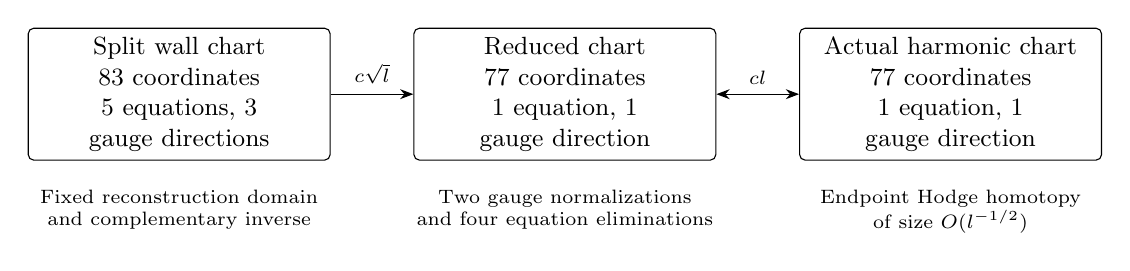
\begin{tikzpicture}[>=Stealth,box/.style={draw,rounded corners=2pt,align=center,text width=3.6cm,minimum height=1.35cm,font=\small}]
\node[box] (wall) {Split wall chart\\$83$ coordinates\\$5$ equations, $3$ gauge directions};
\node[box,right=1.05cm of wall] (finite) {Reduced chart\\$77$ coordinates\\$1$ equation, $1$ gauge direction};
\node[box,right=1.05cm of finite] (harm) {Actual harmonic chart\\$77$ coordinates\\$1$ equation, $1$ gauge direction};
\draw[->] (wall.east)--node[above,font=\scriptsize]{$c\sqrt l$}(finite.west);
\draw[<->] (finite.east)--node[above,font=\scriptsize]{$cl$}(harm.west);
\node[below=0.25cm of wall,align=center,font=\scriptsize] {Fixed reconstruction domain\\and complementary inverse};
\node[below=0.25cm of finite,align=center,font=\scriptsize] {Two gauge normalizations\\and four equation eliminations};
\node[below=0.25cm of harm,align=center,font=\scriptsize] {Endpoint Hodge homotopy\\of size $O(l^{-1/2})$};
\end{tikzpicture}
\end{adjustbox}
\caption{Three descriptions of the same positive-parameter deformation germ.
The arrow labels are sufficient radii about the endpoint for the indicated
operations. The left-hand chart itself has a fixed domain as $l\to0$.
The scalar equations are identified analytically, including higher terms.}
\label{fig:charts}
\end{figure}


The deformation equations used below are summarized in Table~\ref{tab:charts}.
The selected coefficients describe the four-arrow subfamily; the other
four rows describe complete local deformations. In the wall and endpoint
harmonic models, the real curvature equation selects the corrected HE
representatives. The selected family is first balanced quadratically and
then corrected. Neither normalization introduces another holomorphic chart.
\begin{table}[htbp]
\centering\small
\begin{tabular}{@{}>{\raggedright\arraybackslash}p{.23\textwidth}>{\raggedright\arraybackslash}p{.17\textwidth}>{\raggedright\arraybackslash}p{.36\textwidth}>{\raggedright\arraybackslash}p{.12\textwidth}@{}}
\toprule
Presentation & Coordinate & Equation and contraction & Section\\
\midrule
Selected extensions & $z=(A,C,B,D)$ & Five quadratic equations $\Omega=0$;
current split Hodge primitive & \ref{sec:geometry}\\[3pt]
Endpoint \v Cech model & $t\in\CC^{77}$ & Scalar $F(t)=0$;
explicit \v Cech contraction & \ref{sec:endpoint-deformations}\\[3pt]
Endpoint harmonic model & $t\in V_*$ & Scalar $f_*(t)=0$;
actual endpoint Hodge contraction & \ref{sec:endpoint-metric}\\[3pt]
Split wall model & $x\in V\simeq\CC^{83}$ & Five equations $\kappa(x)=0$;
fixed split Hodge contraction & \ref{sec:wall-chart}\\[3pt]
Reduced wall model & $v\in V_l\simeq\CC^{77}$ & Scalar $f_l(v)=0$;
two gauge and four equation eliminations & \ref{sec:transition}\\
\bottomrule
\end{tabular}
\caption{The coordinate presentations and their defining equations.
The symbol $t$ is local to the two endpoint constructions. In Section~\ref{sec:transition},
the actual harmonic obstruction is denoted $F_e$ to distinguish it from
the reduced wall equation $f_l$.}
\label{tab:charts}
\end{table}

\subsection{The estimate and an explicit boundary distance}
The metric proof separates two operations. First eliminate the
infinite-dimensional gauge complement, where a fixed Poincar\'e gap
is available. Harmonic orthogonality makes the harmonic part of the reconstruction
derivative orthogonal to its correction. Its angle with the complementary
gauge range is $O(|x|)$, so orthogonal projection loses only
$O(|x|^2)$ of the squared norm. The corrected HE metric changes it
by another relative $O(|x|^2)$. The result is a positive Hermitian
form on the entire coefficient space, uniformly close to the harmonic
one. Apply this estimate to every $v-C_x\xi$ and only then minimize
over $\xi$. No inverse of the finite orbit operator is required.
Section~\ref{sec:relative} states this argument with explicit hypotheses
for general compact stabilizers, so it can also be used in matrix
multiplicity problems.

To turn that estimate into the geometric theorem one must still prove
coverage, compact-orbit uniqueness and existence of smooth quotient
pieces. We do so using the full holomorphic slice, the normalization
$P_0\log H=0$, and a closed adapted two-form that tames the coefficient
complex structure. We use its moment identity without assuming that
it is a Kähler form. The same positivity proves that finite intrinsic
lengths separate distinct quotient points.

The selected diamond family provides a calculable consequence.
An orbit parameter $M\to\infty$ approaches $W\oplus F_3$ through
regular stable bundles. One transverse squared tangent norm is
$(l-\delta)/(M^2+2)$ to relative $O(l)$, where
$\delta\sim\sqrt{3/5}\,l/M$. A different coordinate,
$r=M^{-1/2}$, extends the balanced family smoothly to the endpoint.
Its finite horizontal speed has squared leading value $2l\sqrt{3/5}$.
Section~\ref{sec:selected-metrics} proves the actual selected-family
distance formula
\begin{equation}\label{eq:intro-distance}
 d_{\mathrm{HE}}(E(M),E_*)=
 \sqrt{2l\sqrt{3/5}}\,M^{-1/2}\bigl(1+O(M^{-1}+l)\bigr).
\end{equation}
The error is uniform in unrelated limits $l\to0$, $M\to\infty$.
At fixed $l$ the leading coefficient is known to relative $O(l)$.
The distance uses paths in the selected local family, not shortcuts
through the larger complete moduli germ.

\subsection{Relation to earlier work}
Buchdahl--Schumacher construct equivariant analytic Kuranishi models
and prove the local polystability correspondence near a fixed HE
bundle \cite{BuchdahlSchumacher20}. Their results supply the qualitative
fixed-endpoint framework. Clarke--Tipler \cite{ClarkeTipler24} and
Delloque \cite{Delloque25} develop local wall-crossing and continuity
with respect to the background metric using complementary reduction
and an adapted finite curvature equation. We use these mechanisms
and prove the fixed-domain estimates and chart transitions required
by the present full threefold deformation space.

The harmonic moduli metric is the standard Weil--Petersson metric of
\cite[Section~4.1]{BiswasSchumacher16}, divided here by the base volume.
Its positivity is on effective Kodaira--Spencer directions. The relation
to the real unitary-connection norm has the explicit factor two stated
in Section~\ref{sec:endpoint-metric}.

The order of quotient elimination and the basic relative minimization
principle already appear in \cite{WuebbenRelativeMetrics26}, which
proves relative $L^2$ metric estimates across reducible Yang--Mills
surface strata. That paper also treats local intrinsic completions.
The present contribution is the higher-dimensional integrable geometry:
a complete convergent obstruction equation with explicitly computed
higher-order terms in the chosen coordinates, a uniform wall chart,
its quantitative transition to actual endpoint harmonic coordinates,
and the realization of the relative estimate on the full local HE
quotient. The stationary construction for the selected three-step
family is taken from \cite{wuebben2026three} with its scope restated
in Section~\ref{sec:geometry}. Complete deformation and quotient
arguments are proved here.

Manetti's formal contraction theorem \cite{manetti2005} is used only
at the formal step of the explicit endpoint calculation; convergence
and analytic comparison are proved separately. The comparison gauges
also identify the harmonic tangent metrics, connecting the deformation
calculation to the relative metric theorem.

% Source: sections/02_geometry.tex
\section{The family and its reducible endpoint}\label{sec:geometry}

Our example is a bundle on a threefold. It has a small family of
three-step presentations, a larger complete deformation space, and a
reducible endpoint at which both the automorphism group and the obstruction
rank change. These are distinct phenomena. We first describe the smaller
family explicitly; its relation with the full moduli problem will then
be visible in coordinates.

\subsection{Fixed geometry and conventions}
Let $X=(\PP^1)^3$, with Fubini--Study forms $\omega_i$ of integral one,
and put
\begin{equation}\label{eq:lines}
 F_1=\cO(-2,-2,4),\quad F_2=\cO(1,-2,1),\quad
 F_3=\cO(-2,1,1),\quad F_4=\cO,\qquad E_0=\bigoplus_iF_i.
\end{equation}
Give the lines their product metrics and $E_0$ their orthogonal sum
$h_0$. Write $d$ for the split Dolbeault differential, on the bundle
or its endomorphisms as indicated by the argument. Block $ij$ means
$\Hom(F_j,F_i)$. The four factors have equal slope for
$\omega_0=\omega_1+\omega_2+\omega_3$.

For small real $k,l$ define
\begin{equation}\label{eq:polarization}
 \omega_{k,l}=h_1\omega_1+h_2\omega_2+\omega_3,\qquad
 h_1=\left(1+\frac{k+5l}{24\pi}\right)^{-1},\quad
 h_2=\left(1+\frac{5k+l}{24\pi}\right)^{-1}.
\end{equation}
The volume is $h_1h_2$. Every $L^2$ inner product below is divided
by this volume. Hermitian products are linear in their second argument;
the associated real metric is their real part. The centered slope differences,
with $\kappa_i=2\pi\deg(F_i)/\Vol$ and
$\kappa_E=\frac14\sum_i\kappa_i$, are
\begin{equation}\label{eq:slope-demands}
 b_i=\kappa_E-\kappa_i,\qquad
 b=\tfrac18(5(k+l),3k-5l,-5k+3l,-3(k+l)).
\end{equation}
Our full wall chart uses the path $k=3l/5$, $0\le l\le l_0$.
We write $\omega_l$ for this path. Then
$b=l(1,-2/5,0,-3/5)$. A separate selected-family result retains
all small $k,l>0$.

Write $(s_i:t_i)$ for homogeneous coordinates and $(s:t)=(s_3:t_3)$.
Let $S_j=H^0(\PP^1_3,\cO(j))$ and
$U_i=H^0(\PP^1_i,\cO(1))$. Choose $e_{0,i}=t_i,e_{1,i}=s_i$,
a class $\theta_i\in H^1(\cO(-2))$, and its Serre-dual harmonic
classes $\eta_i^0,\eta_i^1\in H^1(\cO(-3))$, so that
$\eta_i^je_{m,i}$ has harmonic projection $\delta_{jm}\theta_i$.
All factors are pulled back to $X$ and constant tensor factors are
suppressed. The selected harmonic coordinates are
\begin{align}
 A&=\eta_1^0a_0+\eta_1^1a_1\in V_{12}=U_1^*\otimes S_3,
 &C&=\eta_2^0c_0+\eta_2^1c_1\in V_{13}=U_2^*\otimes S_3,
 \notag\\
 B&=(e_{0,1}b_0+e_{1,1}b_1)\theta_2\in V_{24}=U_1\otimes S_1,
 &D&=\theta_1(e_{0,2}d_0+e_{1,2}d_1)\in V_{34}=U_2\otimes S_1.
 \label{eq:selected-coordinates}
\end{align}
Thus $A,C$ are pairs of cubics, $B,D$ pairs of linears, and the
four dimensions are $8,8,4,4$.

\subsection{The nonlinear relation and the stationary input}
Let $K_h=d_h^*G_h$ be the split Hodge homotopy. Define
\begin{equation}\label{eq:selected-reconstruction}
 N_h(z)=AE_{12}+CE_{13}+BE_{24}+DE_{34}+\Gamma_h(z)E_{14},\qquad
 \Gamma_h=-K_h(A\wedge B+C\wedge D).
\end{equation}
Here $z=(A,C,B,D)$; each $E_{ij}$ records the block only.
The endpoint line $F_1F_4^{-1}$ has $H^1=0$ and
$H^2=\CC(\theta_1\wedge\theta_2)\otimes S_4$.
There are no products of length three. Hodge decomposition therefore gives
\begin{equation}\label{eq:selected-obstruction}
 (d+N_h(z))^2=(\theta_1\wedge\theta_2)\Omega(z)E_{14},\qquad
 \Omega=a_0b_0+a_1b_1-c_0d_0-c_1d_1.
\end{equation}
The minus sign orders the two differential legs by projective-line factor.
The endpoint primitive is part of the bundle, even when a path's harmonic
product vanishes. These identities hold on the entire coefficient space,
and $d_h^*N_h=0$ there.

The effective torus $T=(\CC^*)^4/\CC^*$ acts by $g_i/g_j$ on
block $ij$; $T_c=(S^1)^4/S^1$ is its compact form. On zero-sum
vectors $\xi\in\CC^4$, its infinitesimal action is
\begin{equation}\label{eq:selected-orbit}
 C_z\xi=((\xi_1-\xi_2)A,(\xi_1-\xi_3)C,
             (\xi_2-\xi_4)B,(\xi_3-\xi_4)D).
\end{equation}
For $w=(\|A\|_h^2,\|C\|_h^2,\|B\|_h^2,\|D\|_h^2)$,
write $\mu_h(z)=\mathsf Dw$, where
\begin{equation}\label{eq:incidence}
 \mathsf D=\begin{pmatrix}1&1&0&0\\-1&0&1&0\\
 0&-1&0&1\\0&0&-1&-1\end{pmatrix}.
\end{equation}
We call $z$ quadratically balanced if $\mu_h(z)=b$.
This is twice the usual quadratic moment map for the real part of the
harmonic Hermitian form, with its level multiplied by the same factor.
It changes neither the level set nor the quotient metric convention.

We use the following stationary result of \cite{wuebben2026three}.
On the ambient selected ball, the complementary curvature equation has a
unique small solution $u(h,z)$ perpendicular to real constant diagonals,
with $\|u\|_{C^m}\le C_m\|z\|_h^2$. The remaining equation is
\begin{equation}\label{eq:stationary-cut}
 F(h,z)=-b+\mu_h(z)+R(h,z),\qquad
 |R_S(h,z)|\le C\|z\|_h^2
          \sum_{e\text{ crossing }S}\|z_e\|_h^2.
\end{equation}
Here $R_S=\sum_{i\in S}R_i$. Define the cut energy
$q_{\partial S}=\sum_{e\text{ crossing }S}\|z_e\|_h^2$.
The bound holds for every vertex subset and every ambient coefficient
point, whether or not its obstruction vanishes. It also holds after a diagonal derivative:
if $\dot z_{ij}=(Y_i-Y_j)z_{ij}/2$, then
\begin{equation}\label{eq:stationary-cut-derivative}
 |(D_YR[Y])_S|\le C\|z\|_h^2
       \sum_{e\text{ crossing }S}\|z_e\|_h^2\,\|Y\|_\infty.
\end{equation}
For connected integrable support admitting positive balance, the actual
fixed-determinant HE metric satisfies
$e^{-C\sigma}h_{\rm bal}\le H\le e^{C\sigma}h_{\rm bal}$,
where $\sigma$ is total balanced energy. The constants do not depend on
positive edge ratios. The same ambient zero-form argument identifies
holomorphic endomorphisms with diagonal constants on support components.
These are the precise stationary inputs used below; quotient tangent norms
require the separate argument of Section~\ref{sec:relative}.

\subsection{A sequence with a reducible limit}
Choose normalized cubic monomials $p,q$ proportional to $s^3,t^3$
and a normalized linear monomial $\ell$ proportional to $s$. The
normalizations include their harmonic factors in
\eqref{eq:selected-coordinates}. The two path products have equal
normalization, since polarization weights cancel around the diamond.
For $M\ge0$ take
\begin{equation}\label{eq:M-family}
 A=(p,Mp+q),\qquad C=(p,0),\qquad B=D=(\ell,0).
\end{equation}
Both products in \eqref{eq:selected-obstruction} equal $p\ell$.
Variations of $a_0$ span $\ell S_3$, while a variation of $b_1$
in the complementary linear direction supplies a nonzero $t^4$ term.
Thus $D\Omega$ has rank five at every finite $M$.
The invariant norm ratio is $\rho=M^2+2$.

On $k=3l/5$, the positive balanced representatives are
\begin{align}
 A^0&=\sqrt{\frac{l-\delta}{M^2+2}}(p,Mp+q),&
 C^0&=\sqrt\delta(p,0),\notag\\
 B^0&=\sqrt{3l/5-\delta}(\ell,0),&
 D^0&=\sqrt\delta(\ell,0),\label{eq:balanced-M}
\end{align}
where the unique root in $0<\delta<3l/5$ satisfies
\begin{equation}\label{eq:delta-equation}
 (M^2+2)\delta^2=(l-\delta)(3l/5-\delta).
\end{equation}
The cycle identity verifies both the relation and the diagonal orbit.
As $M\to\infty$, $M\delta/l\to\sqrt{3/5}$, and the limit is
\begin{equation}\label{eq:endpoint-coefficients}
 A_*=(0,\sqrt l\,p),\qquad B_*=(\sqrt{3l/5}\,\ell,0),
 \qquad C_*=D_*=0.
\end{equation}
Its bundle splits as $E_*=W\oplus F_3$, where $W$ has graded
lines $F_1,F_2,F_4$, both adjacent classes nonzero, and the retained
quadratic endpoint primitive.

\begin{proposition}\label{prop:endpoint}
For every sufficiently small $l>0$, $W$ is stable at $\omega_l$ and
has the same slope as $F_3$. The endpoint is polystable,
$\operatorname{Aut}(E_*)=(\CC^*)^2$, and it has an HE metric
$H_*$ with $e^{-Cl}h_0\le H_*\le e^{Cl}h_0$ in the balanced
presentation. Fixing the determinant on each summand fixes its metric
scales.
\end{proposition}
\begin{proof}
On support $\{12,24\}$ the complementary solution and connection
split off $F_3$, by equivariance and uniqueness. Its curvature component
is exactly $-b_3=0$. On $\{1,2,4\}$ the positive weights are
$l,3l/5$, with demand $(l,-2l/5,-3l/5)$.
Restrict diagonal logarithms to $Y_3=0$, $Y_1+Y_2+Y_4=0$.
The cut argument in \eqref{eq:stationary-cut} corrects this balance
by $O(l)$: on a sphere $\|Y\|_\infty=Al$, sort its three values
and use a cut across a largest gap. The moment increment pairs positively
with the cut by at least $cAl$ times its positive cut energy; the residual
is at most $Cl$ times the same energy. For fixed large $A$ and small
$l$ there is no boundary zero. The quadratic moment map has positive
radial pairing, hence degree one; the homotopy to $F$ has the same degree.
This constructs the metric with the asserted bound.

The ambient zero-form estimate gives just one constant endomorphism
on each connected component. Thus $W$ is simple. An HE bundle is an
orthogonal sum of stable equal-slope factors, so simplicity makes $W$
stable; see \cite[Theorem~5.8.3]{Kobayashi87}. The third demand
is zero, proving equality of slopes. The same endomorphism calculation
gives the stated automorphisms. The independent positive scalars are
parallel and do not change the Chern connection; separate determinant
normalizations remove them.
\end{proof}

\subsection{The selected slice and its five pieces}\label{subsec:five-pieces}
For fixed $l>0$, fix the nonzero $s^3$ coefficient of $a_1$ and
$s$ coefficient of $b_0$ by two independent torus characters, to values
$\alpha,\beta$. The residual $H=\CC^*$ acts as
$(C,D)\mapsto(\lambda^{-1}C,\lambda D)$. Put $L=b_0=\beta s+\beta_1t$.
The pair $(L,t)$ is a basis. Write
\begin{align*}
 a_1&=(\alpha/\beta^3)L^3+\gamma_1L^2t+\gamma_2Lt^2+x t^3,
 &b_1&=\eta L+y t,\\
 c_i&=P_i(L,t)+u_it^3,&d_i&=e_iL+v_it\quad(i=0,1),
\end{align*}
where $P_i$ uses $L^3,L^2t,Lt^2$ only.
Division by $L$ solves four equations for $a_0$ and leaves
\begin{equation}\label{eq:selected-quadric}
 xy=u_0v_0+u_1v_1,\qquad
 a_0=-\frac{a_1b_1-c_0d_0-c_1d_1-(xy-u_0v_0-u_1v_1)t^4}{L}.
\end{equation}
The numerator is identically divisible. Thus the slice is
$\CC^4\times\{xy=u_0v_0+u_1v_1\}\subset
\CC^4\times\CC^2\times\CC^8\times\CC^4$,
of dimension $17$, with $18$-dimensional tangent at its origin.
The four extra neutral variables are $\beta_1,\gamma_1,\gamma_2,\eta$.
The six displayed quadratic variables vanish precisely on its singular
locus, of dimension $12$; equivalently $D\Omega$ then has rank four.

Let $W_{jm}=C_jD_m$ be the $8$ by $4$ invariant matrix. Its relations
are the $2$ by $2$ minors, since invariant monomials pair negative and
positive weights. The quotient germ is
\begin{equation}\label{eq:selected-quotient}
 \CC^4\times\{(x,y,W):\rk W\le1,\quad
 xy=W_{u_0v_0}+W_{u_1v_1}\}.
\end{equation}
The closed orbits have both $C,D$ nonzero or both zero. A one-sided
orbit has the neutral point in its closure. A closed orbit meets the
quadratic moment level uniquely modulo $T_c$: in full support its weights
are $(l-\delta,\delta,3l/5-\delta,\delta)$, where the invariant ratio
uniquely determines $\delta$; on the two-edge support, the two characters
set the norms to $l$ and $3l/5$. These representatives remain local.
Indeed residual scaling gives $\|C\|=\|D\|=\sqrt{\|W\|}$,
so $C,D\to0$ as $W\to0$, and the positive scales on the nonzero
$A,B$ edges tend to one.

Put $Z_6=(x,y,u_0,u_1,v_0,v_1)$. The following are smooth complex
pieces of this selected quotient:
\begin{center}
\begin{adjustbox}{max width=\textwidth,center}
\begin{tabular}{lccc}
\toprule
Closed representative & Dimension & Stabilizer & $\rk D\Omega$\\
\midrule
$C,D\ne0$, $Z_6\ne0$ &16&$1$&5\\
$C,D\ne0$, $Z_6=0$ &11&$1$&4\\
$C=D=0$, $x\ne0$, $y=0$ &5&$\CC^*$&5\\
$C=D=0$, $x=0$, $y\ne0$ &5&$\CC^*$&5\\
$C=D=0$, $x=y=0$ &4&$\CC^*$&4\\
\bottomrule
\end{tabular}
\end{adjustbox}
\end{center}
For the second row the charged dimensions are $6$ and $2$, giving
$6+2-1+4=11$; the other dimensions follow from
\eqref{eq:selected-quadric}. The first two rows are stable. In the last
three the bundle is $W_z\oplus F_3$, with $W_z$ stable by the proof
of Proposition~\ref{prop:endpoint}. The two five-dimensional branches
meet on the four-dimensional piece.

These points are actual isomorphism classes. On full support the
reference-slope socle is $F_1$ and the socle of its quotient is
$F_2\oplus F_3$: cross-line Hom groups vanish and the two adjacent
extensions on each side are nonzero. Every isomorphism preserves this
filtration and induces four scalar maps; it acts by exactly the torus
characters on the adjacent classes. Conversely those characters give an
isomorphism, including the endpoint primitive. This is the orbit
classification in \cite[Section~6]{wuebben2026three}. On the reducible
locus the stable decomposition distinguishes $W_z$ from $F_3$, and
its reference-slope socle filtration distinguishes $F_1,F_2,F_4$.
The same argument gives exactly the two active characters. A stable
bundle cannot be isomorphic to a reducible one.
The complete deformation problem is substantially larger than these five
pieces, as we now show.

% Source: sections/03_endpoint_deformations.tex
\section{The complete deformation equation at the endpoint}\label{sec:endpoint-deformations}

The selected slice has eighteen infinitesimal directions at $E_*$.
The full fixed-determinant space has seventy-seven. We compute the missing
directions and give a convergent equation that retains their interactions.
The quadratic term is particularly simple, but it does not replace the
complete equation.

\subsection{A finite complex computing the endpoint cohomology}
For this calculation fix $l>0$ and rescale the two nonzero extension
classes by a constant diagonal, so they are
$A=\eta_1^1s^3$ and $B=e_{0,1}\theta_2s$.
This is a holomorphic normalization; its metric bounds are allowed to
depend on $l$. On the three affine factors use coordinates
$\xi=s_1/t_1$, $\eta=s_2/t_2$, $\zeta=s/t$.
The one-factor \v Cech complex for $\cO(d)$ is
\begin{equation}\label{eq:cech-complex}
 C^0(d)=\CC[\xi]\oplus\xi^d\CC[\xi^{-1}],\qquad
 C^1(d)=\CC[\xi,\xi^{-1}],\qquad
 d(f_0,f_1)=f_1-f_0.
\end{equation}
For the ordered cup product, use the first-chart component in degree
$(0,1)$, the second-chart component in degree $(1,0)$, and componentwise
multiplication in degree $(0,0)$. Products of two degree-one cochains
on one factor vanish. Take the tensor product over the three factors,
with Koszul signs and matrix composition. Products pair the appropriate
Hom bundles; a single line-bundle complex is not an algebra by itself.

The inclusion $i$ sends a degree-zero cohomology monomial to both charts
and a degree-one monomial to the intersection. The projection $p$ reads
the second-chart coefficients $0\le e\le d$ in degree zero and retains
$d<e<0$ in degree one. On a degree-one monomial set
\begin{equation}\label{eq:cech-homotopy}
 h(\xi^e)=
 \begin{cases}
 (-\xi^e,0),& e\ge0,\\
 (0,\xi^e),&e<0\text{ and }e\le d,\\
 0,&d<e<0.
 \end{cases}
\end{equation}
It is zero in degree zero. Direct substitution gives
$dh+hd=1-ip$, $hi=ph=h^2=0$, and $pi=1$.
On the tensor product use
$h_1\otimes1\otimes1+i_1p_1\otimes h_2\otimes1+
 i_1p_1\otimes i_2p_2\otimes h_3$, with tensor signs.
These formulas also recover projective-line cohomology and K\"unneth;
see \cite[Tags~01XT and 0BED]{stacks}.

In this complex the endpoint is
\begin{equation}\label{eq:cech-endpoint}
 A=i(\xi^{-2}\zeta^3E_{12}),\quad
 B=i(\eta^{-1}\zeta E_{24}),\quad
 \Gamma=-h(AB),\qquad N=A+B+\Gamma.
\end{equation}
Here $p(AB)=0$, so $d\Gamma=-AB$ and $dN+N^2=0$.
For an explicit descent check, put $A_0=\xi^{-2}\zeta^3$,
$B_0=\eta^{-1}\zeta$. The correction on a $\xi$ edge is
$1+A_0E_{12}$. On an $\eta$ edge it is $1+B_0E_{24}$ in the
first $\xi$ chart and $1+B_0E_{24}-A_0B_0E_{14}$ in the second.
The two square products both equal $1+A_0E_{12}+B_0E_{24}$.
The third-coordinate twists are $3,1,4$. Thus these invertible
triangular transitions glue the endpoint bundle. Its central lift is
unique up to gauge because $H^1(F_1)=0$, so it agrees with
\eqref{eq:selected-reconstruction}.
For endomorphisms the edge differential $Gu_1-u_0G$ becomes the
usual transition-conjugated differential after multiplication by $G^{-1}$;
the square identity gives the same identification in higher degrees.

Set $d_N=d+\delta$, where
$\delta u=Nu-(-1)^{\deg u}uN$. The transferred operators are
\begin{equation}\label{eq:finite-transfer}
 I=(1+h\delta)^{-1}i,\quad P=p(1+\delta h)^{-1},\quad
 K'=h(1+\delta h)^{-1},\qquad \partial=p\delta I.
\end{equation}
Every inverse here is a finite sum. Give the four factors heights
$(2,1,1,0)$. Multiplication by an adjacent endpoint arrow raises
matrix-block height by one and multiplication by $\Gamma$ raises it
by two; the Hom-block heights range from $-2$ to $2$.
The homotopy preserves blocks. Expanding the finite sums using
$dh+hd=1-ip$ and $d_N^2=0$ gives
\[
 d_NI=I\partial,\quad Pd_N=\partial P,\quad
 d_NK'+K'd_N=1-IP,\quad PI=1.
\]
Thus this finite complex computes all endpoint cohomology, including
blocks outside the original filtration.

The split cohomology is
\begin{center}
\begin{adjustbox}{max width=\textwidth,center}
\begin{tabular}{lcc}
\toprule
Hom block & $h^1$ & $h^2$\\
\midrule
$12,13,21,31,23,32$ & $8$ each & $0$\\
$24,34$ & $4$ each & $0$\\
$41$ & $27$ & $0$\\
$14$ & $0$ & $5$\\
\bottomrule
\end{tabular}
\end{adjustbox}
\end{center}
Every off-diagonal $H^0$ and every $H^3$ vanish; four diagonal
constants remain. The split dimensions are $(4,83,5,0)$.
The image of $\partial_0$ is $\operatorname{span}(A,B)$, of rank two.
On the adjacent blocks,
\begin{equation}\label{eq:endpoint-differential}
 \partial_1(\dot A,\dot C,\dot B,\dot D)
       =\zeta\dot a_0+\zeta^3\dot b_1\in S_4.
\end{equation}
Its image is $sS_3$, of dimension four. There is only one additional
arrow on a path from an adjacent input to block $14$, so this formula
is exact, rather than a first-order truncation of the transfer.

The omitted blocks give zero to every order. Indeed the residual scalar
on $F_3$ has nonzero character on $13,23,31,32,34$, whereas the target
$14$ is neutral. Rotate the third coordinate, compensating on the lines
by weights $(4,1,0,0)$. A block-$ij$ monomial of exponent $e$ has
weight $e+u_j-u_i$. The background and all transfer operators preserve
this weight. The remaining omitted blocks $21$ and $41$ have strictly
positive weights, respectively $1,2$ and $1,2,3$; the target weights
are $-4,-3,-2,-1,0$. Their images must vanish.
Consequently
\begin{equation}\label{eq:endpoint-cohomology}
 (h^0,h^1,h^2,h^3)(\End_0E_*)=(1,77,1,0).
\end{equation}
Removing the scalar only changes degree zero, since $H^{>0}(\cO_X)=0$.

The residual effective scalar acts on $H^1$ with decomposition
\begin{equation}\label{eq:character-decomposition}
 V_*=V_0\oplus V_-\oplus V_+,\qquad
 (\dim V_0,\dim V_-,\dim V_+)=(41,16,20).
\end{equation}
The neutral blocks $12,21,24,41$ have $47$ coordinates before removing
two gauge and four equation directions. Blocks $13,23$ have weight
$-1$ and dimensions $8+8$; blocks $31,32,34$ have weight $+1$ and
dimensions $8+8+4$.
The selected tangent injects with character dimensions $(6,8,4)$.
Its complementary $59$ directions are represented by corrected classes
from blocks
\begin{equation}\label{eq:omitted-directions}
 V_{21}\oplus V_{41}\oplus V_{23}\oplus V_{31}\oplus V_{32},
 \qquad\dim=(8,27,8,8,8).
\end{equation}
Their actual cocycles are obtained with $I$, not by using uncorrected
split forms.

\subsection{An explicit convergent scalar equation}
We now specify every coefficient of the full obstruction, including its
higher terms. In the transferred degree-one complex retain all split
monomials except the four $a_0$ monomials and the two background
monomials $A,B$. Replace the two $b_1$ monomials by
\begin{equation}\label{eq:endpoint-basis}
 \xi\eta^{-1}\zeta^jE_{24}-\xi^{-1}\zeta^{j+2}E_{12},
 \qquad j=0,1.
\end{equation}
These $77$ vectors define a cohomology inclusion $j_1$.
In degree two use $j_2(1)=\xi^{-1}\eta^{-1}E_{14}$.
A second homotopy on the finite complex is zero except for
\begin{equation}\label{eq:second-homotopy}
 k(A)=-E_{11},\qquad k(B)=E_{44},\qquad
 k(\xi^{-1}\eta^{-1}\zeta^{j+1}E_{14})
       =\xi^{-1}\zeta^jE_{12}\quad(0\le j\le3).
\end{equation}
In degree zero retain the constant on $\{1,2,4\}$ and the constant
on $\{3\}$. If $\pi$ reads cohomology in these complements,
then $\partial k+k\partial=1-j\pi$. Hence
\begin{equation}\label{eq:endpoint-contraction}
 J=Ij,\qquad\Pi=\pi P,\qquad K=K'+IkP
\end{equation}
satisfy $d_NK+Kd_N=1-J\Pi$, $K^2=KJ=\Pi K=0$, and $\Pi J=1$.
All these operators are fixed at the endpoint.

For $t\in V_*$ define homogeneous cochains and scalar polynomials by
\begin{equation}\label{eq:full-recursion}
 a_1(t)=Jt,\quad c_n(t)=\sum_{i=1}^{n-1}a_i(t)a_{n-i}(t),\quad
 a_n(t)=-Kc_n(t),\quad F_n(t)=\Pi c_n(t)\quad(n\ge2).
\end{equation}
In degree two $\Pi$ is the scalar coefficient of
$\xi^{-1}\eta^{-1}E_{14}$. Each coefficient in this recursion is
obtained by finite Laurent operations with rational coefficients.

\begin{theorem}\label{thm:endpoint-base}
The series $F=\sum_{n\ge2}F_n$ converges near zero in $V_*$.
Its zero germ is a fixed-determinant semiuniversal deformation base of
$E_*$, of dimension $76$. It is invariant under the scalar action
with weights $0,-1,+1$ in \eqref{eq:character-decomposition}.
In the specified raw coordinates its quadratic term is
\begin{equation}\label{eq:full-quadratic}
 F_2=xy-u_0v_0-u_1v_1,
\end{equation}
of rank six and radical dimension $71$. The selected family is its
intersection with the linear $18$-dimensional selected coordinate space.
The complete base contains a transverse $35$-dimensional family of
polystable bundles and has regular stable quotient charts of dimension $75$.
\end{theorem}

\begin{proof}
We first prove convergence and analytic semiuniversality, then compute the
quadratic term and the selected restriction. The final part constructs
the transverse polystable family and the regular stable charts.
For convergence complete the cochain spaces in the weighted Laurent norm
\[
 \left\|\sum_e c_e\xi^{e_1}\eta^{e_2}\zeta^{e_3}\right\|_R
 =\sum_e|c_e|R^{|e_1|+|e_2|+|e_3|},\qquad R>1.
\]
The chart exponent conditions are those of \eqref{eq:cech-complex}.
These series are holomorphic on the corresponding discs and exterior
discs, with annular intersections. Cup multiplication is bounded because
$R^{|e+f|}\le R^{|e|}R^{|f|}$. The monomial projections and homotopies,
multiplication by $N$, finite transfer sums and finite-dimensional second
contraction are bounded. If $M$ bounds $K$ composed with multiplication,
the scalar majorant $v=u+Mv^2$, $u=\|Jt\|$, converges for $4Mu<1$.
It majorizes \eqref{eq:full-recursion} and proves convergence of
\begin{equation}\label{eq:endpoint-fixedpoint}
 a(t)=Jt-K(a(t)^2),\qquad F(t)=\Pi(a(t)^2).
\end{equation}
For $c=d_Na+a^2$ the contraction and Bianchi identities give
\[
 c=JF+K(ca-ac).
\]
Smallness makes the last operator have norm less than one. Thus $F=0$
is equivalent to the full Maurer--Cartan equation. The perturbed
transitions remain invertible in a norm controlling their sup norms on
smaller charts, and therefore glue actual holomorphic bundles.

Gauge fixing in degree zero uses parameters in $\im K$ to impose
$Ka=0$. Its derivative there is $\pm Kd_N=\pm1$, so the analytic
implicit-function theorem gives the slice. The remaining coordinate has
identity Kodaira--Spencer differential on $H^1$. The formal contraction
argument supplies a hull, as in \cite[Proposition~4.6 and Theorem~4.7]{manetti2005};
convergence has just been proved separately.
For analytic completeness one may compare with the full Dolbeault
Kuranishi construction at the fixed endpoint. Its Green contraction and
complex gauge fixing are bounded between Sobolev spaces of sufficiently
high order. Passing from transitions to smooth Dolbeault operators and
then fixing this gauge gives a holomorphic map of the two zero germs,
with identity derivative on $H^1$ and an isomorphism of formal hulls.
Extend its coordinate functions to the ambient analytic germs. The
inverse-function theorem makes this an ambient coordinate change.
The completed defining ideals agree; faithful flatness of completion
for a Noetherian local ring \cite[Tag~00MC]{stacks} implies that their
analytic ideals agree. The local rings of convergent power series are
Noetherian. This proves analytic semiuniversality, including the defining
ideal rather than just the reduced zero set.

The determinant imposes no new equation: $H^1(\cO_X)=H^2(\cO_X)=0$
and $\operatorname{Pic}(X)$ is discrete. Locally identify the determinant
by taking logarithms of its transition ratios and solving the scalar
\v Cech cocycle; normalize by a local fourth root. This removes the scalar
automorphism only. All contraction operators respect the residual action,
so $F$ is invariant.

The raw coordinates in \eqref{eq:full-quadratic} are the coefficients of
\begin{center}
\begin{adjustbox}{max width=\textwidth,center}
\begin{tabular}{cl}
\toprule
Coordinate & Transferred cohomology vector\\
\midrule
$x$ & $\xi^{-2}E_{12}$\\
$y$ & $\xi\eta^{-1}E_{24}-\xi^{-1}\zeta^2E_{12}$\\
$u_0,u_1$ & $\eta^{-1}E_{13},\ \eta^{-2}E_{13}$\\
$v_0,v_1$ & $\xi^{-1}E_{34},\ \xi^{-1}\eta E_{34}$\\
\bottomrule
\end{tabular}
\end{adjustbox}
\end{center}
Substitution in $\Pi((Jt)^2)$ gives the three pairs with coefficients
$1,-1,-1$. There are no other quadratic pairs. One can see the
vanishing on omitted directions directly from the weights: the target
has third-coordinate weight $-4$. Omitted neutral directions have
positive weights, while selected neutral weights are at least $-3$.
The omitted negative-character block $23$ has weight $-1$; omitted
positive-character blocks $31,32$ have weights $2,3$ and $1$.
The selected negative and positive weights are respectively $-4,\ldots,-1$
and $0,1$. No pair involving an omitted direction has both residual
weight zero and third-coordinate weight $-4$.

All contractions preserve the selected subalgebra of constant diagonals
and blocks $12,13,24,34,14$. Its gauge condition fixes the two original
nonzero coefficients, and $H^1(F_1)=0$ fixes the central lift up to gauge.
Consequently zero omitted coordinates give precisely the selected
family, and conversely that family can be normalized inside this
subalgebra. Its adapted coordinates give \eqref{eq:selected-quadric};
the raw recursive coordinates agree to first order and may differ at
higher order.

On $V_{21}\oplus V_{41}$ every coordinate has positive third weight,
so no monomial can contribute to the obstruction of weight $-4$.
Thus $F$ vanishes there to all orders and analytically. Reconstruction
uses only the $W$ blocks, giving $W_t\oplus F_3$.
At fixed $l$, the trace-free HE linearization on stable $W$ is invertible.
The implicit-function theorem gives nearby HE metrics; openness of
simplicity makes $W_t$ stable. Its slope is unchanged, hence these are
polystable bundles. Their Kodaira--Spencer map is injective on this
$35$-dimensional space, transverse to the selected tangent. The stable
$W$ slice identifies distinct sufficiently near parameters with distinct
bundles.

Finally the quadratic initial term of $F$ cannot factor into two
linear forms, because its rank is six. Therefore the convergent germ
$F$ is irreducible and its zero set has dimension $76$.
The regular stable selected points \eqref{eq:M-family} approach the
endpoint; their nonzero selected equation derivative makes $dF\ne0$.
Stability is open at fixed polarization. The residual scalar action is
free there, and fixing one nonzero charged coordinate gives a local
$75$-dimensional stable quotient chart. The complementary gauge
linearization is $Kd_a=1+K[a,\cdot]$ on $\im K$, still invertible
on a small ball, so no further infinitesimal gauge direction is lost.
\end{proof}

\subsection{Higher terms that the quadratic equation does not record}
For a concrete restriction of the recursion, retain the following five
raw parameters:
\[
 x:\xi^{-2}E_{12},\quad
 y:\xi\eta^{-1}E_{24}-\xi^{-1}\zeta^2E_{12},\quad
 r:\xi^{-2}\zeta E_{12},\quad
 b:\eta^{-1}E_{24},\quad c:\xi^3\zeta^{-2}E_{21}.
\]
Apply $I$ to these vectors to obtain their endpoint cocycles. The last
parameter is outside the selected family. Equations
\eqref{eq:cech-homotopy}--\eqref{eq:full-recursion} give
\begin{equation}\label{eq:higher-terms}
 F_2=xy,\qquad F_3=-r(by+cx),\qquad
 F_4=-b^3y+bcr^2.
\end{equation}
For example, the cubic is
$-\Pi(a_1K(a_1^2)+K(a_1^2)a_1)$; the quartic is
\[
 \Pi\bigl(a_1K(a_1K(a_1^2)+K(a_1^2)a_1)
 +K(a_1K(a_1^2)+K(a_1^2)a_1)a_1+K(a_1^2)K(a_1^2)\bigr).
\]
The printed monomial rules determine every coefficient of these expressions.
They illustrate a higher interaction with an omitted direction.
They do not prove an intrinsically nonquadratic singularity: solving the
critical $x,y$ pair gives $x=br+O(3)$, $y=cr+O(3)$, and the residual
quartic cancels, $bcr^2-(br)(cr)=0$. The complete convergent equation,
rather than a proposed analytic normal form, is the deformation model
used in the metric arguments.

% Source: sections/04_endpoint_metric.tex
\section{The complete metric germ at fixed polarization}\label{sec:endpoint-metric}

Fix $l>0$ sufficiently small. The endpoint $E_*=W\oplus F_3$
has an HE metric $H_*=H_W\oplus H_3$, with the determinant of each
summand fixed separately. We first construct the metric germ using its
actual harmonic representatives. Constants in this section may depend
on $l$. This dependence will be resolved by a different chart in
Sections~\ref{sec:wall-complex}--\ref{sec:wall-chart}.

\subsection{Harmonic coordinates and the remaining scalar equation}
Let $D$ be the Dolbeault differential on $\End_0E_*$ and let
$\Pi_q,G_q$ be its harmonic projections and Green operators. The
calculation of Section~\ref{sec:endpoint-deformations} identifies
\[
 V_*=\cH^1_D=V_0\oplus V_-\oplus V_+,
 \qquad (\dim V_0,\dim V_-,\dim V_+)=(41,16,20),
 \qquad \dim\cH^2_D=1.
\]
The effective group $H=\CC^*$ acts with weights $0,-1,+1$.
Its Hermitian trace-free generator and infinitesimal orbit map are
\begin{equation}\label{eq:endpoint-generator}
 T_* =\diag(-\tfrac14 I_W,\tfrac34 I_{F_3}),\quad
 \|T_*\|^2=\tfrac34,\qquad
 C_t\xi=\xi(0,-t_-,t_+).
\end{equation}
These three subspaces are orthogonal in the volume-normalized harmonic
norm. Relative rescaling of $H_W,H_3$ changes the cross-summand norms;
our fixed choice is part of the coordinates.

For an integer $s\ge6$, solve in $H^s$
\begin{equation}\label{eq:endpoint-kuranishi}
 a_*(t)=t-D^*G_2(a_*(t)\wedge a_*(t)),\qquad
 f_*(t)=\Pi_2(a_*(t)\wedge a_*(t)).
\end{equation}
Sobolev multiplication and the order-minus-one homotopy give a
convergent analytic solution on a small ball. Its correction $b_*=a_*-t$
satisfies
\begin{equation}\label{eq:endpoint-reconstruction-bounds}
 \Pi_1b_*=D^*b_*=0,\qquad
 \|b_*(t)\|_{H^s}\le C_l|t|^2,\qquad
 \|D_tb_*v\|_{H^s}\le C_l|t|\,|v|.
\end{equation}
The curvature identity and Bianchi identity imply that $D+a_*(t)$ is
integrable exactly when $f_*(t)=0$: the remaining curvature satisfies
an equation $c=\Pi_2c+K(ca_*-a_*c)$, whose last operator has norm less
than one. The construction commutes with $H$. The analytic comparison
in Section~\ref{sec:endpoint-deformations} identifies this scalar equation
with its complete \v Cech equation, up to an invertible analytic factor
and an equivariant analytic change of coordinates. In particular no
higher obstruction terms are removed in passing to $f_*$.

Let $P_*$ be the real orthogonal projection onto $\RR T_*$ and
$Q_*=1-P_*$. On $Q_*$ the endpoint operator $D^*D$ has a positive
gap $\gamma_l$. For every small $t$, including nonintegrable ones,
form the compatible unitary connection from $D+a_*(t)$ and a metric
$H_*e^u$, transported by $e^{u/2}$ to $H_*$. Write its centered mean
curvature as $\mathcal M_*(u,t)$. At zero its $u$ derivative is
$D^*D$; its $t$ derivative is zero by $D^*a_*=0$. The real analytic
implicit-function theorem gives
\begin{equation}\label{eq:endpoint-complement}
 Q_*\mathcal M_*(u_*(t),t)=0,\quad P_*u_*=0,\quad
 \|u_*(t)\|_{H^{s+1}}\le C_l|t|^2.
\end{equation}
Define
\[
 m_*(t)=\langle\mathcal M_*(u_*(t),t),T_*\rangle.
\]
On $f_*^{-1}(0)$ the metric $H(t)=H_*e^{u_*(t)}$ is HE exactly
when $m_*(t)=0$.

\subsection{Correction relative to charged energy}
The neutral coordinates may be much larger than the charged ones.
An absolute Taylor estimate for $m_*$ is therefore insufficient.
Put $\rho_*(t)=|t_-|^2+|t_+|^2$ and
$m_2(t)=|t_+|^2-|t_-|^2$.

\begin{lemma}\label{lem:charged-remainder}
On an ambient ball of radius $r$,
\begin{equation}\label{eq:charged-remainder}
 |m_*-m_2|\le C_l r\rho_*,\qquad
 |E(m_*)-2\rho_*|\le C_l r\rho_*,\quad
 E=(0,-t_-,t_+).
\end{equation}
In particular these estimates do not require a lower bound for
$\rho_*/r^2$.
\end{lemma}
\begin{proof}
The quadratic part of $m_*$ is the sum of block norms multiplied by
target-minus-source eigenvalues of $T_*$. This is exactly $m_2$.
The linear curvature of $b_*$ has zero $T_*$ projection, and
$D^*Du_*$ does also, so there is no other quadratic term.
On the neutral subspace the reconstructed connection and its corrected
metric preserve $W\oplus F_3$. The integrated partial trace on each
summand equals its degree. Their slopes coincide, hence $m_*(t_0,0)=0$,
including when $f_*(t_0,0)\ne0$. This uses a compatible unitary
connection, not a nonexistent holomorphic structure off the zero set.
Circle invariance makes the first derivative in charged directions
zero at every neutral point.

Thus $R=m_*-m_2$ vanishes to second order in the charged variables,
and its full quadratic jet at zero vanishes. On the radius-$r$ ball
its charged second derivative is $O_l(r)$. Taylor's integral formula
in those variables gives $|R|\le C_lr\rho_*$. Differentiating the
same formula along $E$ gives the second bound. All derivatives are
taken before restriction to the obstruction locus.
\end{proof}

\begin{proposition}\label{prop:endpoint-balance}
Every sufficiently small closed $H$ orbit in $f_*^{-1}(0)$ has a
representative with $m_*=0$, unique up to the compact circle within
the local construction. The closed orbits are exactly those with both
$t_-,t_+$ nonzero and those with both zero. In the first case, after
flat balance $|t_-|=|t_+|$, the further positive gauge has logarithm
$O_l(r)$. These orbits give stable bundles. The neutral orbits give
the nearby polystable decompositions $W_t\oplus F_3$.
\end{proposition}
\begin{proof}
For weights $0,-1,+1$, an orbit with both charged components nonzero
is closed, as is a neutral point. A one-sided orbit has the neutral
point in its closure. These assertions follow directly by considering
$\lambda\to0,\infty$; a sequence with neither behavior has a
convergent subsequence in $\CC^*$.

If $a=|t_-|>0$ and $b=|t_+|>0$, the real gauge
$s_0=\frac12\log(a/b)$ makes both norms equal to $\sqrt{ab}$.
It decreases their sum of squares, so stays in the coordinate ball.
Starting there, Lemma~\ref{lem:charged-remainder} gives a residual
$O_l(r)\rho_*$ and a derivative at least $\rho_*$ on a sufficiently
small interval. The intermediate value theorem gives a unique zero
with $|s|\le C_lr$. Monotonicity gives local uniqueness. On the
neutral subspace $m_*$ is identically zero; on a one-sided orbit its
sign is that of $m_2$, by the same relative estimate.

The local polystability correspondence for deformations of an HE bundle
identifies closed automorphism orbits with polystable bundles
\cite[Theorems~5.4 and 8.1]{BuchdahlSchumacher20}. We use it at
the fixed endpoint and fixed polarization. The HE metrics have also
been constructed directly above. A holomorphic endomorphism in this
small slice is determined by its parallel part: applying $D^*$ to its
endomorphism equation and absorbing the small coefficient terms forces
its complementary part to vanish. Equivariance then identifies the
endomorphism algebra with the stabilizer of $t$. A charged closed orbit
has no effective stabilizer, so its polystable bundle is stable.
A neutral deformation preserves the two summands; the rank-three one
remains stable after shrinking the neighborhood. This also follows from
its unchanged scalar endomorphism algebra and its constructed HE metric.
\end{proof}

The analytic quotient retains the full equation $f_*$. Its invariant
coordinates are $t_0$ and the $16$ by $20$ matrix
$t_-\otimes t_+$, subject to the $2$ by $2$ minors and to the descended
analytic obstruction ideal. To see that this description is analytic,
expand an invariant convergent power series in charged monomials.
Every invariant monomial pairs the same number of negative and positive
variables, hence factors into entries of that matrix. On a smaller
polydisc the absolute majorant remains convergent. This argument does
not replace the obstruction by its quadratic term.

\subsection{The harmonic quotient metric}
For $t$ with $f_*(t)=m_*(t)=0$ and $v\in\ker Df_{*,t}$, set
\begin{align}
 g_{*,\mathrm{fin}}([v])
 &=\inf_{\xi\in\CC}|v-C_t\xi|^2,\label{eq:endpoint-finite}\\
 g_{*,\mathrm{HE}}([v])
 &=\inf_\zeta\|D_ta_*v-(D+[a_*,\cdot])\zeta\|_{H(t),l}^2.
 \label{eq:endpoint-he}
\end{align}
The latter is the volume-normalized harmonic Kodaira--Spencer norm.
It is $\Vol_l^{-1}$ times the Weil--Petersson convention of
\cite[Section~4.1]{BiswasSchumacher16}. A real unitary-connection
variation has squared norm twice its Hermitian $(0,1)$ norm; all
lengths here use $\operatorname{Re}g_{\mathrm{HE}}$.

\begin{theorem}\label{thm:endpoint-metric}
On every smooth complex piece of this local polystable quotient,
\begin{equation}\label{eq:endpoint-relative}
 (1-C_lr^2)g_{*,\mathrm{fin}}\le g_{*,\mathrm{HE}}
 \le(1+C_lr^2)g_{*,\mathrm{fin}}.
\end{equation}
The exact Kodaira--Spencer kernel is $\im C_t$. The constants are
independent of the positive charged energy and of nonzero singular
values of $Df_*$. The assertion includes the complete $75$-dimensional
regular stable charts and the neutral polystable subfamilies constructed
in Section~\ref{sec:endpoint-deformations}.
\end{theorem}
\begin{proof}
Apply Theorem~\ref{thm:relative} with the endpoint as reference,
$\mathfrak g=\CC T_*$, and $q=|t|^2$. Equations
\eqref{eq:endpoint-reconstruction-bounds} give harmonic orthogonality
of the derivative correction. Equivariance gives
$(D+[a_*,\cdot])\xi=-D_ta_*C_t\xi$. The fixed endpoint Poincar\'e
estimate gives complementary coercivity; \eqref{eq:endpoint-complement}
gives the metric bound. All hypotheses are now verified, with constants
depending only on the fixed endpoint. No inverse of $C_t$ occurs.
At a charged point the finite form can also be written
\[
 |v|^2-\frac{|\langle v,(0,-t_-,t_+)\rangle|^2}{\rho_*};
\]
on the neutral piece there is no subtraction. The two expressions
refer to their respective tangent spaces, not to arbitrary vectors
in a common coarse Zariski tangent space.
\end{proof}

This theorem alone does not control $l\to0$. The reference gap and
the harmonic reconstruction constants may deteriorate. The next
section computes that deterioration, and the following two sections
construct a chart in which the elliptic gap remains fixed.

% Source: sections/05_wall_complex.tex
\section{The endpoint deformation complex at the wall}\label{sec:wall-complex}

The endpoint harmonic space has dimension $77$, whereas the split
harmonic space has dimension $83$. The difference comes from two gauge
directions and four equation directions that disappear from cohomology
for $l>0$. Their eigenvalues all tend to zero with $l$. We compute them
before choosing coordinates for the wall neighborhood.

\subsection{A smooth normalization of the endpoint}
Put $\tau=\sqrt l$, and retain the fixed split Hodge contraction
$(\iota,P,K)$ at $\omega_0$. Write
\begin{equation}\label{eq:endpoint-path}
 A^o=\eta_1^1s^3E_{12},\quad B^o=e_{0,1}\theta_2sE_{24},\quad
 a_l=\|A^o\|_l^{-1},\quad b_l=\sqrt{3/5}\,\|B^o\|_l^{-1},\quad
 \alpha_l=a_lA^o+b_lB^o.
\end{equation}
Here $a_l,b_l$ are positive normalizing constants; the subscript on a
polynomial coordinate such as $\dot a_0$ has a different meaning.
Product harmonic representatives are independent of the positive
polarization coefficients. Indeed the product Laplacian is the sum
of commuting factor Laplacians with positive scalar multipliers.
Consequently $a_l,b_l$ are smooth in $l$.

An integrable fixed-reference presentation of the endpoint is
\begin{equation}\label{eq:wall-endpoint-operator}
 N_\tau=\tau\alpha_l-\tau^2K(\alpha_l^2),\qquad
 D_\tau=d+[N_\tau,\cdot].
\end{equation}
There is only the composable pair $12,24$, its harmonic product is
zero, and no longer product occurs. Thus $dN_\tau+N_\tau^2=0$.
Replacing $K$ by the current homotopy $K_l$ changes the central
entry by an exact form. Since $K_l-K=O(l)$ and the product has
size $\tau^2$, the gauge $1+\phi_\tau E_{14}$ identifying the two
presentations has $\phi_\tau=O(\tau^4)$ in every fixed smooth norm.
The sign is fixed by $g(d+N)g^{-1}$; explicitly $d\phi_\tau$ is
the old central entry minus the new one.

The endpoint HE metric can be chosen smoothly in $\tau$, with logarithm
$O(\tau^2)$ relative to $h_0$. To prove the needed regularity, use the
complementary metric solution of \eqref{eq:stationary-cut} and vary
a diagonal $Y$ with $Y_3=0$, $Y_1+Y_2+Y_4=0$. Its reduced equation is
\[
 -\tau^2(1,-2/5,0,-3/5)
       +\mu_l(e^Y\tau\alpha_l)+R(l,e^Y\tau\alpha_l)=0.
\]
The remainder is $O(\tau^4)$, smoothly in $\tau,Y$. Taylor's integral
formula divides the equation smoothly by $\tau^2$. At zero its
$Y$ derivative is positive definite on the indicated two-dimensional
space, with quadratic form a positive multiple of
\[
 |Y_1-Y_2|^2+\tfrac35|Y_2-Y_4|^2.
\]
The ordinary implicit-function theorem gives $Y(\tau)=O(\tau^2)$.
The third curvature component is identically zero. Together with
the complementary solution and the central gauge, this proves the
claim in every fixed smooth order. Separate determinant normalization
on $W,F_3$ removes the remaining constant rescaling. Transport by
the metric isometry to $h_0$ changes the differential only by
$O(\tau^2)$, so the actual endpoint differential is
$d+\tau[\alpha_0,\cdot]+O(\tau^2)$.

\subsection{A bounded finite complex}
Let $\delta_\tau=[N_\tau,\cdot]$. Heights $(2,1,1,0)$ on the
four factors make $\delta_\tau$ strictly increase block height,
whereas $K,P$ preserve it. Hence
\begin{equation}\label{eq:wall-finite-transfer}
 I_\tau=(1+K\delta_\tau)^{-1}\iota,\quad
 P_\tau=P(1+\delta_\tau K)^{-1},\quad
 K_\tau=K(1+\delta_\tau K)^{-1},\quad
 \partial_\tau=P\delta_\tau I_\tau
\end{equation}
are finite Neumann sums. Expanding $dK+Kd=1-\iota P$ gives
\begin{gather}
 D_\tau I_\tau=I_\tau\partial_\tau,\quad
 P_\tau D_\tau=\partial_\tau P_\tau,\quad P_\tau I_\tau=1,
 \notag\\
 D_\tau K_\tau+K_\tau D_\tau=1-I_\tau P_\tau.
 \label{eq:wall-contraction}
\end{gather}
All these maps are uniformly bounded in fixed Sobolev orders, and
$K_\tau$ gains one derivative. They retain the small finite differential
rather than inverting it.

The fixed trace-free harmonic dimensions are $(3,83,5,0)$ by the
cohomology table in Section~\ref{sec:endpoint-deformations}. On these
spaces the exact nonzero maps are
\begin{align}
 \partial_\tau\xi
 &=\tau a_l(\xi_2-\xi_1)A^o+
                \tau b_l(\xi_4-\xi_2)B^o,\notag\\
 \partial_\tau(\dot A,\dot C,\dot B,\dot D,\ldots)
 &=\tau(b_ls\dot a_0+a_ls^3\dot b_1)
       \quad\hbox{in }S_4.\label{eq:wall-finite-differential}
\end{align}
The first formula follows because $K\delta_\tau\xi=0$ and the
quadratic central term has zero harmonic projection. For the selected
adjacent blocks only one further arrow can lead to the target $14$,
which gives the second formula without higher terms.

There are no omitted columns in the second map. Blocks incident to
vertex $3$ have nonzero character under its residual scalar, whereas
$14$ is neutral. For the remaining blocks $21,41$, rotate the third
projective coordinate and compensate by line weights $(4,1,0,0)$.
A monomial of third exponent $e$ in block $ij$ has weight
$e+u_j-u_i$. The weights of $21$ and $41$ are respectively
$\{1,2\}$ and $\{1,2,3\}$, while the target weights are
$\{-4,-3,-2,-1,0\}$. The endpoint and the contraction commute
with this circle, so every term in \eqref{eq:wall-finite-transfer}
preserves weights. This proves the all-orders vanishing.

For $\tau>0$, the ranks are two and four, with degree-one image
$sS_3\subset S_4$. Their composite is zero: the first map changes
$a_1,b_0$, not $a_0,b_1$. The cohomology is therefore exactly
$(1,77,1,0)$. Let $d_1$ denote \eqref{eq:wall-finite-differential}
with the factor $\tau$ removed and $l=0$.

\begin{proposition}\label{prop:wall-low-complex}
The actual endpoint Dolbeault Laplacians in degrees $0,1,2,3$ have
smooth low spectral subspaces of dimensions $(3,83,5,0)$ on
$0\le\tau<\tau_0$. Their complementary Green operators are uniformly
bounded $H^m\to H^{m+2}$ for each fixed $m$. For $\tau>0$ the
low positive eigenvalue counts are $(2,6,4,0)$; every such eigenvalue
satisfies
\begin{equation}\label{eq:wall-low-eigenvalues}
 \lambda_j(l)/l=c_j+O(\sqrt l),
\end{equation}
where the positive constants in degree zero are
$(8-\sqrt{19})/5,(8+\sqrt{19})/5$, those in degree two are
$6/25,12/25,28/25,64/25$, and those in degree one are their union.
The zero multiplicities are exactly $(1,77,1,0)$.
\end{proposition}
\begin{proof}
Use the smooth endpoint normalization and the smooth form and density
isometries to put all operators on fixed $L^2$ spaces with common
$H^2$ domains. Their difference from the split Laplacian is
$O(\tau):H^2\to L^2$. Choose a contour surrounding zero below the
split positive spectrum. The resolvent Neumann series converges there,
so the Riesz projections $\Pi_{\tau,q}$ are smooth and have ranks
$(3,83,5,0)$. The complements have one positive uniform gap.
That gap and elliptic regularity give their asserted Green estimates.

The differential commutes with the successive Laplacians. Polar
normalization of $\Pi_{\tau,q}\iota$ identifies the low spaces
isometrically with the fixed harmonic spaces. In those identifications
the finite differential is $\tau d_1+O(\tau^2)$: derivatives of
the identifications multiplied by $d$ vanish after harmonic projection.
Thus the low Laplacian is
$\tau^2(d_1^*d_1+d_1d_1^*)+O(\tau^3)$.
Finite-dimensional min--max proves \eqref{eq:wall-low-eigenvalues}.
The exact cohomology computed above identifies all remaining low
modes as zero, so no smaller positive eigenvalues are hidden in the
error term.

For the constants, in the coordinate $z=s/t$ use
\[
 \theta=\frac{d\bar z}{(1+|z|^2)^2},\qquad
 \eta^0=\frac{2d\bar z}{(1+|z|^2)^3},\qquad
 \eta^1=\frac{2\bar z\,d\bar z}{(1+|z|^2)^3}.
\]
The Fubini--Study normalization gives $|d\bar z|^2=2\pi(1+|z|^2)^2$.
A beta integral yields
\[
 \|s^jt^{d-j}\|^2=((d+1)\tbinom dj)^{-1},\qquad
 \|\theta\|^2=2\pi,\qquad \|\eta^j\|^2=4\pi.
\]
Consequently $\|A^o\|^2=\pi$, $\|B^o\|^2=\pi/2$,
$a_0=\pi^{-1/2}$ and $b_0=\sqrt{6/(5\pi)}$.
The zero-form operator is the three-vertex path of weights $1,3/5$
plus the isolated vertex. Its two positive eigenvalues are the stated
ones. In degree two the monomials $s^jt^{4-j}$ are orthogonal, and
$d_1d_1^*$ has entries
\[
 \frac{4}{5\binom4j}
 \left(\frac65\binom3{j-1}+2\mathbf1_{j\ge3}\right),
 \qquad 1\le j\le4.
\]
They are the four printed rational constants. Hodge decomposition of
the finite complex gives their union with the two degree-zero constants
in degree one.
\end{proof}

The actual endpoint homotopy $D_\tau^*G_{\tau}$ therefore has norm
at most $C/\tau$ from $H^m$ to $H^{m+1}$, while its harmonic
projections remain uniformly bounded. On the low spaces this follows
from the singular values of the differential, and on their complements
from the uniform elliptic bounds. In contrast, the homotopy $K_\tau$
in \eqref{eq:wall-finite-transfer} is uniformly bounded because it
does not contract those finite directions. This distinction explains
both the larger wall chart and the shrinking domain of its transition
to the endpoint harmonic chart.

% Source: sections/06_wall_chart.tex
\section{A complete deformation chart with a fixed domain}\label{sec:wall-chart}

We now keep all split harmonic directions. The resulting chart has
$83$ coordinates, five obstruction components and three effective
diagonal gauge directions. Its elliptic inverse and its domain remain
fixed as $l\to0$. Kuranishi reconstruction and complementary metric
reduction are standard local tools; the point here is to retain the
entire collapsing finite complex of Proposition~\ref{prop:wall-low-complex}.

\subsection{Reconstruction and exact integrability}
Let $V=\cH^1_d$, $O=\cH^2_d$, with dimensions $83$ and $5$.
All Hodge operators in this subsection use the fixed split reference.
There are holomorphic maps on a fixed ball $B_{r_0}\subset V$
\begin{equation}\label{eq:wall-reconstruction}
 a(x)=\iota x-K(a(x)\wedge a(x)),\qquad
 \kappa(x)=P_2(a(x)\wedge a(x)).
\end{equation}
To specify their convergence, let $I_s$ bound harmonic inclusion into
$H^s$, $s\ge6$, and let $M$ dominate the bilinear norms of
$K(\cdot\wedge\cdot)$ in $H^s$ and $H^{s-1}$. Choose
$8MI_sr_0<1/2$. The first map in \eqref{eq:wall-reconstruction}
contracts the $H^s$ ball of radius $2I_s|x|$. Equivalently,
\[
 a_1=\iota x,\qquad
 a_n=-K\sum_{j=1}^{n-1}a_j\wedge a_{n-j}\quad(n\ge2)
\]
has a convergent Catalan majorant. This specifies all higher terms.
The trace of a square of an endomorphism-valued one-form is zero,
so the trace-free condition is preserved.

Write $J_x=D_xa$. Differentiation gives
\begin{equation}\label{eq:wall-derivative}
 J_xv=\iota v-K(J_xv\wedge a+a\wedge J_xv).
\end{equation}
The inverse on the right has norm at most two. In particular
\begin{equation}\label{eq:wall-reconstruction-bounds}
 \|a-\iota x\|_{H^s}\le C|x|^2,\qquad
 \|J_xv-\iota v\|_{H^s}\le C|x|\,|v|,
\end{equation}
and second derivatives are uniformly bounded on a smaller ball.
Elliptic regularity gives any fixed higher spatial order after a
corresponding fixed decrease of radius.

For the full curvature $c=da+a^2$, Hodge decomposition and Bianchi give
\begin{equation}\label{eq:wall-curvature-identity}
 c=\iota\kappa+K(c\wedge a-a\wedge c).
\end{equation}
The last operator has norm less than one in $H^{s-1}$. Thus
$\kappa=0$ is equivalent to full integrability. Constant diagonals
commute with the contraction, so reconstruction and obstruction are
$T$-equivariant whenever both coordinates lie in the domain.
The group need not preserve the ball.

\subsection{Completeness and all isomorphisms}
For any small perturbation $b$ of $d$, use a complex gauge $e^v$,
with $v$ perpendicular to the reference harmonic zero-forms, to impose
\[
 d^*\bigl(e^v\cdot(d+b)-d\bigr)=0.
\]
The derivative in $v$ is $-d^*d:H^{s+1}\to H^{s-1}$ on this
fixed complement. Its inverse is bounded. The analytic implicit-function
theorem gives a gauge and bounded first derivatives on one fixed
neighborhood. If $b$ is integrable, its Coulomb representative $b'$
satisfies $b'=\iota P_1b'-K(b'^2)$, so $b'=a(x)$.
This proves completeness, including deformations that do not preserve
the selected three-layer filtration.

\begin{lemma}\label{lem:wall-orbit-converse}
Every holomorphic bundle map between two sufficiently small integrable
members $d+a(x),d+a(y)$ is a constant diagonal. Consequently two such
members are isomorphic exactly when $y=gxg^{-1}$ for $g\in T$.
No bound on the size of the isomorphism is required.
\end{lemma}
\begin{proof}
In the full endomorphism space decompose a holomorphic map as
$g=g_0+g_1$, where $g_0$ is a constant diagonal and $g_1$ is
orthogonal to the four diagonal constants. Its equation is
\[
 dg_1+a(y)g_1-g_1a(x)+a(y)g_0-g_0a(x)=0.
\]
Since $g_0$ is parallel and both reconstructed forms are co-closed,
applying $d^*$ kills the last two terms. Pairing with $g_1$ gives
\[
 \|dg_1\|^2\le C(\|a(x)\|_\infty+\|a(y)\|_\infty)
                   \|dg_1\|\,\|g_1\|.
\]
The fixed Poincar\'e inequality forces $g_1=0$ on one sufficiently
small ball. Harmonic projection then gives $yg_0=g_0x$.
For an isomorphism all diagonal entries are nonzero, giving the
$T$ action after removing the common scalar. Conversely equivariance
makes every such diagonal an isomorphism. The proof never estimates
$\|g_0\|$.
\end{proof}

This is the co-closed-slice mechanism of
\cite[Proposition~4.5 and Corollary~4.6]{BuchdahlSchumacher20}.
That source's quadratic reconstruction estimate is used for harmonic
input, as in its equation~(2.4); an estimate for arbitrary nonclosed
one-forms is unnecessary here. The direct argument above proves the
precise converse needed in this chart. Continuous gauge fixing gives
local inverses on orbit spaces. This assertion retains nonclosed
orbits and makes no Hausdorff claim for their unseparated quotient.

The point $x_l=\tau\alpha_l$ satisfies $a(x_l)=N_\tau$.
For small $l$, it lies in $B_{r_0/4}$. Thus one fixed chart contains
a fixed-radius neighborhood of every moving endpoint, in the fixed
smooth presentation. This follows from completeness about $d$ and
the triangle inequality, not from an endpoint inverse with a collapsing
gap.

\subsection{The complementary HE equation}
For a trace-free $h_0$-Hermitian $u$, form the compatible unitary
connection of $d+a(x)$ and $h_0e^u$, transported to $h_0$ by
$e^{u/2}$. Denote it by $A(l,x,u)$ and put
\[
 \mathcal M(l,x,u)=i\Lambda_lF_{A(l,x,u)}-\kappa_E(l)I.
\]
The fixed determinant connection has constant mean curvature, so this
expression is pointwise trace-free. Let $P_0$ project onto real
constant trace-free diagonals, and $Q_0=1-P_0$. The normalized
zero-form measure is the fixed product measure, so these projections
do not vary with $l$.

At $x=u=0$ the curvature is $-b(l)$, and its $Q_0$ projection
vanishes. Its metric derivative is
\[
 \tfrac12(\Delta_{\partial,l}+\Delta_{\db,l}).
\]
The quadratic form is the sum of two derivative energies; its kernel
on Hermitian zero-forms is exactly the constant diagonals. The fixed
gap and ellipticity give a uniformly bounded inverse on
$Q_0H^{s+1}\to Q_0H^{s-1}$. The parameter implicit-function theorem
therefore gives a smooth $T_c$-equivariant map $u(l,x)$ on a fixed
product neighborhood, with
\begin{equation}\label{eq:wall-metric-complement}
 Q_0\mathcal M(l,x,u(l,x))=0,\quad P_0u=0,\quad
 \|u(l,x)\|_{H^{s+1}}\le C|x|^2,\quad
 \|D_xu(l,x)v\|_{H^{s+1}}\le C|x|\,|v|.
\end{equation}
Indeed $u(l,0)=0$, and the first $x$ derivative vanishes because
all split harmonic one-forms remain harmonic for $\omega_l$.
The Sobolev elliptic inverse gives the usual complementary reduction in
\cite[Section~3]{ClarkeTipler24} and
\cite[Lemma~4.1 and Proposition~4.2]{Delloque25}, with a fixed
reference complement containing no collapsing modes.

Define the remaining real equation and the adapted connection by
\begin{equation}\label{eq:wall-moment}
 m_l(x)=P_0\mathcal M(l,x,u(l,x)),\qquad
 \Phi_l(x)=A(l,x,u(l,x)).
\end{equation}
The slope term $m_l(0)=-b(l)$ is retained. The equations
$\kappa(x)=0$, $m_l(x)=0$ are precisely the integrable HE equations
in this normalization. The holomorphic family $d+a(x)$ supplies
the complex geometry; $\Phi_l$ is a smooth real family.

For completeness among nearby HE pairs, first use the preceding
complex gauge fixing and transport the metric to the holomorphic
slice. In an $h_0$-orthonormal frame, a further real constant diagonal
$Y$ imposes
\begin{equation}\label{eq:metric-normalization}
 P_0\log(e^{-Y}He^{-Y})=0.
\end{equation}
Its derivative in $Y$ at $H=I,Y=0$ is $-2\id$, so the
finite-dimensional implicit-function theorem has uniform bounds.
The corresponding action $e^Yx$ preserves the holomorphic slice.
Uniqueness in the complementary equation now identifies the metric
with $h_0e^{u(l,e^Yx)}$.

Finally the selected $24$-dimensional subspace is an exact restriction
of the complete chart. Its products have only the central block $14$,
and further products vanish. Hence its recursion terminates as
\eqref{eq:selected-reconstruction}, with $K$ replacing $K_h$, and
its obstruction is precisely \eqref{eq:selected-obstruction}.
The central gauge changing $K$ to $K_l$ has bounds
$O(l|x|^2)$ and derivative $O(l|x|)$. It follows by applying $K$
to the closed difference of the two primitives. The full chart itself
is not restricted to this subspace and its recursion need not terminate.

% Source: sections/07_chart_transition.tex
\section{The transition to endpoint harmonic coordinates}\label{sec:transition}

At every $l>0$ the larger chart can be reduced to the endpoint
chart. The reduction has two different scales. Four finite equations
can be eliminated on a ball of radius $c\sqrt l$; a controlled comparison
with the actual harmonic chart is obtained on a ball of radius $cl$.
The following theorem collects the two comparisons. Its proof occupies
the three subsections below.

\begin{theorem}\label{thm:chart-transition}
Let $0<l\le l_0$, $\tau=\sqrt l$, and let $x_l=\tau\alpha_l$ be
the endpoint in \eqref{eq:wall-endpoint-operator}. There are constants
$c,c',C>0$, independent of $l$, with the following properties.
Fixing the two nonzero coefficients along the endpoint arrows gives an
$81$-dimensional holomorphic slice to the two nonstabilizing diagonal
gauge directions. On this slice, four obstruction equations can be
solved for four coordinates on $|v|<c\sqrt l$. The resulting
$77$-coordinate base is defined by the full scalar equation $f_l(v)=0$
in \eqref{eq:reduced-wall-equation}.

On $|v|<cl$, a gauge imposing the actual endpoint Coulomb condition
defines an analytic coordinate change $t=t_l(v)$ to the actual endpoint
harmonic space. The derivatives of this map and its inverse are bounded
by $C$, and its image contains $|t|<c'l$. If $F_{e,l}$ is the full
endpoint harmonic obstruction, then
\[
 F_{e,l}(t_l(v))=u_l(v)f_l(v),\qquad u_l(v)\ne0.
\]
The maps commute with the residual scalar action and identify the
reconstructed bundles on the zero sets. The displayed radii are
sufficient radii for these conclusions; no optimality is asserted.
\end{theorem}

\subsection{Two gauge normalizations and four equations}
At $x_l=\tau\alpha_l$, differentiate \eqref{eq:wall-reconstruction}.
The exact finite transfer of Section~\ref{sec:wall-complex} gives
\begin{equation}\label{eq:wall-obstruction-linearization}
 D\kappa_{x_l}(\dot x)
 =\tau(b_ls\dot a_0+a_ls^3\dot b_1).
\end{equation}
Its image is $E=sS_3$, with complement $\CC t^4\subset S_4$.
The omitted-block columns vanish exactly by the character argument
already given, rather than just to leading order in $\tau$.

Fix the coefficient of $s^3$ in $a_1$ and that of $s$ in $b_0$
to their endpoint values $\tau a_l,\tau b_l$. These are two
independent characters of $T$. On $|x-x_l|<c\tau$ the coefficients
remain within half their nonzero endpoint values. The required
logarithms of their ratios are bounded, with derivatives at most
$C/\tau$. Their action changes $x$ by at most $C|x-x_l|$.
The remaining group is the scalar $H$ of the isolated third factor.

The resulting affine slice has dimension $81$. Split its tangent as
$V_l\oplus W$, where $W$ is the four-dimensional $a_0$ polynomial
space and $V_l$ is the kernel of \eqref{eq:wall-obstruction-linearization}
inside the slice. Thus in $V_l$
\[
 \dot a_0=-(a_l/b_l)s^2\dot b_1.
\]
The projections and coordinate identifications are uniformly bounded,
since $a_l/b_l$ stays in a compact positive interval. In particular
$\dim V_l=77$. For $x=x_l+v+w$, the four $E$ equations are
\begin{equation}\label{eq:finite-elimination}
 \tau L_lw+R_l(v,w)=0,\qquad L_lw=b_ls\,w,
 \qquad |R_l(v,w)|\le C(|v|+|w|)^2.
\end{equation}
Their derivative remainder is at most $C(|v|+|w|)$.
These bounds follow from the uniformly bounded second derivatives of
$\kappa$. The map $L_l:W\to E$ has a uniformly bounded inverse.
Contraction on $|w|\le C|v|^2/\tau$ therefore gives an analytic
solution for $|v|<c\tau$, with
\begin{equation}\label{eq:finite-elimination-bounds}
 |w_l(v)|\le C|v|^2/\tau,\qquad
 \|Dw_l(v)\|\le C|v|/\tau.
\end{equation}
Choose $c$ so that the contraction derivative is below $1/2$.
The remaining equation is the full scalar function
\begin{equation}\label{eq:reduced-wall-equation}
 f_l(v)=P_{E^\perp}\kappa(x_l+v+w_l(v)).
\end{equation}
We identify its target with $\CC$ by the monomial $t^4$.

All choices are $H$-equivariant, so $f_l$ is invariant. The neutral
blocks $12,21,24,41$ have $47$ coordinates before removal of two
gauge and four equation directions, leaving $41$. Blocks $13,23$
have weight $-1$ and dimension $16$; blocks $31,32,34$ have weight
$+1$ and dimension $20$. This recovers the endpoint character spaces.
The fixed reference slice, the two finite normalizations and
\eqref{eq:finite-elimination} give analytic completeness. The
Kodaira--Spencer map is an isomorphism onto the endpoint $H^1$,
as follows from the exact finite complex. This proves semiuniversality;
the following comparison gives the stronger coordinate assertion.

\subsection{The smaller harmonic comparison domain}
Write $\mathcal H_\tau,\mathcal K_\tau$ for actual endpoint harmonic
projection and Hodge homotopy, in the presentation $d+N_\tau$ with
its normalized HE metric. Proposition~\ref{prop:wall-low-complex}
gives, in every fixed Sobolev order,
\begin{equation}\label{eq:endpoint-hodge-loss}
 \|\mathcal H_\tau\|_{H^m\to H^m}\le C_m,\qquad
 \|\mathcal K_\tau\|_{H^m\to H^{m+1}}\le C_m/\tau.
\end{equation}
Let $J_l=D_xa|_{x_l}$. The linear map
\begin{equation}\label{eq:transition-linear}
 L_\tau:V_l\longrightarrow\cH^1_{D_\tau},\qquad
 L_\tau v=\mathcal H_\tau J_lv
\end{equation}
is uniformly invertible. Indeed the low-complex identifications
converge to the fixed harmonic spaces. In the finite limiting complex,
$V_l$ converges to $\ker d_1$ with the two coefficients along
$A^o,B^o$ removed; those two orthogonal monomials span $\im d_1$
in degree one. It is therefore the finite cohomology representative
space. Projection to it and its inverse stay bounded.

For a small perturbation $b$ of $D_\tau$, impose the endpoint
Coulomb condition by a gauge $e^{v_g}$, with $v_g$ in the degree-zero
image of $\mathcal K_\tau$:
\[
 \mathcal K_\tau\bigl(e^{v_g}\cdot(D_\tau+b)-D_\tau\bigr)=0.
\]
Its $v_g$ derivative at zero is $-\id$. By
\eqref{eq:endpoint-hodge-loss}, the constant term is at most
$C\|b\|/\tau$ and the nonlinear Lipschitz bound is at most
$C(\|b\|+\|v_g\|)/\tau$. Thus on $\|b\|_{H^s}<c\tau^2$
contraction gives
\begin{equation}\label{eq:endpoint-gauge-bound}
 \|v_g(b)\|_{H^{s+1}}\le C\|b\|_{H^s}/\tau,\qquad
 \|Dv_g\|\le C/\tau.
\end{equation}
This is a sufficient domain, not an optimal-radius assertion.

For $b=a(x_l+v+w_l(v))-N_\tau$, define the new harmonic coordinate
\[
 t(v)=\mathcal H_\tau^1
       \bigl(e^{v_g(b)}\cdot(D_\tau+b)-D_\tau\bigr).
\]
Harmonic projection kills the linear term $D_\tau v_g$. The remaining
exponential terms have bounds
$C(\|v_g\|\|b\|+\|v_g\|^2)$, and
\eqref{eq:finite-elimination-bounds} bounds the finite elimination.
Consequently
\begin{equation}\label{eq:transition-estimate}
 |t(v)-L_\tau v|\le C|v|^2/\tau^2,\qquad
 \|Dt(v)-L_\tau\|\le C|v|/\tau^2.
\end{equation}
On a sufficiently small $c\tau^2$ ball the quantitative analytic
inverse-function theorem gives an inverse with uniformly bounded
first derivative; the image contains a $c'\tau^2$ ball. Thus the
coordinate transition and inverse have bounded derivatives on
specified $cl$ neighborhoods.

\subsection{The exact analytic equation identity}
Equality of zero sets would not be enough to identify the complete
obstruction germ. We prove equality of its defining ideals directly.
Let $e=t^4$ denote the fixed obstruction basis, and abbreviate
$a=a(x_l+v+w_l(v))$. Equation~\eqref{eq:wall-curvature-identity} gives
\begin{equation}\label{eq:curvature-factor}
 da+a^2=S(v)f_l(v),\qquad S(v)=(1+K\ad_a)^{-1}\iota e.
\end{equation}
Here $\ad_a$ is the graded commutator. Its sign follows by moving
the last term of \eqref{eq:wall-curvature-identity} to the left.
This inverse is bounded on the fixed reference ball.

Set $g=e^{v_g(b)}$ and $b'=g\cdot(D_\tau+b)-D_\tau$.
Its curvature is $S'f_l$, where $S'=gSg^{-1}$.
On the $c\tau^2$ ball,
\[
 \|b'\|_{H^s}\le C|v|/\tau,\qquad |t|\le C|v|,
 \qquad \|S'\|_{H^{s-1}}\le C.
\]
Let $a_e(t)$ be the complete endpoint reconstruction with homotopy
$\mathcal K_\tau$, and set
\[
 F_e(t)=\mathcal H_\tau^2(a_e(t)^2).
\]
It converges for $|t|<c\tau$, by the bound $C/\tau$ on that
homotopy, with $\|a_e(t)\|_{H^s}\le C|t|$.
The endpoint Coulomb condition and Hodge identity give
\[
 b'=t-\mathcal K_\tau(b'^2)+\mathcal K_\tau S'f_l.
\]
Subtract the recursion for $a_e$. With $z=b'-a_e$,
\[
 z+\mathcal K_\tau(z\wedge b'+a_e\wedge z)
          =\mathcal K_\tau S'f_l.
\]
The operator on the left is invertible because its perturbation has
norm bounded by
\[
 C\tau^{-1}(\|b'\|+\|a_e\|)\le Cc.
\]
Thus $z=B(v)f_l(v)$ with analytic $B$ and $\|B\|_{H^s}\le C/\tau$.
Harmonic projection of the curvature now yields the identity
\begin{equation}\label{eq:analytic-ideal-identity}
 F_e(t(v))=u_l(v)f_l(v),\qquad
 u_l=\mathcal H_\tau^2S'
    -\mathcal H_\tau^2(B\wedge b'+a_e\wedge B).
\end{equation}
Choose the endpoint obstruction coordinate along
$\mathcal H_\tau^2I_\tau e$. At $v=0$ the gauge is the identity,
$b'=a_e=0$ and $S=I_\tau e$, so $u_l(0)$ is nonzero.
Its norm has a uniform positive lower bound: $e$ is perpendicular
to the finite image $sS_3$, and actual harmonic projection converges
to the finite cohomology projection. The preceding estimates give
$|u_l(v)-u_l(0)|\le C|v|/\tau^2$. Decrease the fixed $c$ once
more to make $u_l$ nonvanishing throughout the comparison ball.

Together with the ambient analytic inverse-function theorem,
\eqref{eq:analytic-ideal-identity} identifies the defining ideals in
both directions, including multiplicity. All maps commute with the
residual $H$ action. On the zero sets the displayed gauges identify
the reconstructed bundles. Hence the $77$-coordinate model, the
actual harmonic endpoint model and the explicit \v Cech model of
Section~\ref{sec:endpoint-deformations} describe the same full analytic
germ. In particular its $76$-dimensional base, $35$-dimensional
transverse polystable family and $75$-dimensional regular stable
quotient charts survive the wall-chart reduction. Stability in this
last assertion comes from the fixed-polarization geometric argument,
not from integrability alone.

% Source: sections/08_relative_quotients.tex
\section{A relative estimate before taking the quotient}\label{sec:relative}

The analytic estimate is best proved on the whole coefficient space.
One first removes the uniformly coercive gauge directions. The resulting
positive form differs quadratically from the harmonic coefficient form.
Only then does one minimize over the finite gauge algebra. This order
preserves the estimate even when the finite orbit loses rank.
We formulate the minimization principle of
\cite[Section~4]{WuebbenRelativeMetrics26} with the hypotheses needed
for the present integrable charts and general compact stabilizers.

\subsection{Hypotheses and the two forms}
We state the argument for a general compact complex manifold and a fixed
Hermitian bundle $(E,h_0)$, so that its precise analytic requirements are
visible. Let $d$ be a split Dolbeault operator on $\End_0E$. Let $p$
range over a relatively compact finite-dimensional parameter domain of
inner products on forms. Their spatial norms are uniformly equivalent.
Assume that the normalized measure, the zero-form $L^2$ inner product and the splitting
\[
 L^2(\End_0E)=\mathfrak g\oplus QL^2
\]
are fixed, where $\mathfrak g$ is the complex algebra of parallel
$d$-holomorphic trace-free zero-forms. Let $G$ be its complex gauge group
and $K$ a compact form acting by parallel $h_0$-unitary automorphisms.
Let $V$ be a fixed finite-dimensional harmonic degree-one space, with
inclusion $\iota$ and norm $\|v\|_p=\|\iota v\|_p$.
In every parameter norm,
$\langle\iota v,d\eta\rangle_p=0$.

On one product neighborhood assume the following data. The reconstruction
$a_p(x)$ and obstruction $\kappa_p(x)$ are holomorphic in $x$, smooth in
$p$, and spatially regular enough for the operations below, with
$a_p(x)=O(|x|)$ in $C^0$. They reconstruct an integrable operator
exactly on $\kappa_p^{-1}(0)$. Write
\[
 D_{p,x}=d+[a_p(x),\cdot],\qquad J_{p,x}=D_xa_p.
\]
The first derivative has the orthogonal decomposition
\begin{equation}\label{eq:relative-hypotheses}
 J_{p,x}v=\iota v+B_{p,x}v,\qquad
 \langle\iota w,B_{p,x}v\rangle_p=0,\qquad
 \|B_{p,x}v\|_p\le C|x|\|v\|_p.
\end{equation}
This orthogonality, rather than a first-order bound alone, will give
a quadratic error. The linear $G$ action has infinitesimal orbit map
$C_x:\mathfrak g\to V$. Exact reconstruction equivariance and
differentiated integrability give
\begin{equation}\label{eq:relative-equivariance}
 D_{p,x}\xi=-J_{p,x}C_x\xi,\qquad
 D_{p,x}J_{p,x}v=0\quad
 (\kappa_p(x)=0,\ v\in\ker D\kappa_{p,x}).
\end{equation}
The second identity uses the full obstruction equation.

Assume the split estimate
\begin{equation}\label{eq:relative-coercivity}
 \|\eta\|_{W^{1,2}}\le C\|d\eta\|_p
 \quad(\eta\in QW^{1,2}),
\end{equation}
and smooth $K$-equivariant metrics $H_{p,x}=h_0e^{u(p,x)}$ with
$\|u\|_\infty\le Cq_p(x)$, where $q_p(x)=\|x\|_p^2$.
The metrics are HE on the geometric solution locus. The estimate itself
also makes sense off that locus. Define
\begin{align}
 g_{\rm fin,p,x}([v])
 &=\inf_{\xi\in\mathfrak g}\|v-C_x\xi\|_p^2,
 \label{eq:general-finite}\\
 g_{\rm harm,p,x}([v])
 &=\inf_{\zeta\in W^{1,2}(\End_0E)}
       \|J_{p,x}v-D_{p,x}\zeta\|_{H_{p,x},p}^2.
 \label{eq:general-harmonic}
\end{align}
The brackets mean quotient by $\im C_x$. At an integrable point and
for $v\in\ker D\kappa$, the second expression is the harmonic
Kodaira--Spencer squared norm. Its interpretation as a tangent metric
requires a specified smooth piece of the geometric quotient.

\begin{theorem}\label{thm:relative}
Under these hypotheses, after decreasing the common radius,
\begin{equation}\label{eq:general-relative}
 (1-Cq_p(x))g_{\rm fin,p,x}([v])
 \le g_{\rm harm,p,x}([v])
 \le(1+Cq_p(x))g_{\rm fin,p,x}([v])
\end{equation}
for every ambient $v\in V$. On $\ker D\kappa$ at an integrable point,
the exact kernel of $v\mapsto[J_{p,x}v]$ is $\im C_x$.
There is a smooth positive $K$-equivariant Hermitian form
$\mathcal B_{p,x}$ on $V$ such that
\begin{gather}
 (1-Cq_p(x))\|v\|_p^2\le\mathcal B_{p,x}(v,v)
 \le(1+Cq_p(x))\|v\|_p^2,\label{eq:ambient-positive}\\
 g_{\rm harm,p,x}([v])=
 \inf_{\xi\in\mathfrak g}
 \mathcal B_{p,x}(v-C_x\xi,v-C_x\xi).\label{eq:ambient-quotient}
\end{gather}
No lower bound for a positive singular value of $C_x$ or $D\kappa_{p,x}$
is required. The group need not be abelian.
\end{theorem}

\begin{proof}
Suppress $p,x$. Multiplication by $a$ has norm $O(|x|)$ from
zero-form $L^2$ to one-form $L^2$. Thus \eqref{eq:relative-coercivity}
and absorption give
\begin{equation}\label{eq:deformed-coercivity}
 \|\eta\|_{W^{1,2}}\le C\|D\eta\|_p
 \quad(\eta\in QW^{1,2}).
\end{equation}
In particular $D(QW^{1,2})$ is closed. Orthogonality in
\eqref{eq:relative-hypotheses} gives
$\|Jv\|_p^2=\|v\|_p^2+\|Bv\|_p^2$.
For the angle with that range, expand
\[
 \langle Jv,D\eta\rangle_p
 =\langle Bv,d\eta\rangle_p+
   \langle Jv,[a,\eta]\rangle_p.
\]
The omitted harmonic term vanishes exactly. Each term on the right
is bounded by $C|x|\|v\|_p\|D\eta\|_p$, using
\eqref{eq:deformed-coercivity}; also
$\|d\eta\|_p\le C\|D\eta\|_p$ by the same absorption.
Hence the orthogonal projection of $Jv$ onto $D(QW^{1,2})$ has
norm at most $C|x|\|v\|_p$. Removing it loses the square of that
norm. We obtain, for every $v$,
\begin{equation}\label{eq:before-minimization}
 (1-C|x|^2)\|v\|_p^2
 \le\inf_{\eta\in QW^{1,2}}\|Jv-D\eta\|_p^2
 \le(1+C|x|^2)\|v\|_p^2.
\end{equation}
The metric $h_0e^u$ changes squared endomorphism norms by factors
between $e^{-2\|u\|_\infty}$ and $e^{2\|u\|_\infty}$.
Thus the same estimate holds in $H_{p,x}$.

Let $R_{p,x}$ be the $H_{p,x},p$-orthogonal projection off
$D_{p,x}(QW^{1,2})$ and set
\[
 \mathcal B_{p,x}(v,w)=
 \langle R_{p,x}J_{p,x}v,R_{p,x}J_{p,x}w\rangle_{H_{p,x},p}.
\]
This proves \eqref{eq:ambient-positive}. To justify smoothness, regard
$A=D_{p,x}|_{QW^{1,2}}$ as a map between fixed Hilbert spaces.
Its weak normal operator $A^*A:QW^{1,2}\to(QW^{1,2})^*$ is
uniformly coercive by \eqref{eq:deformed-coercivity}. Its inverse
and the range projection $A(A^*A)^{-1}A^*$ therefore depend smoothly
on the parameters. All ingredients are $K$-equivariant.
Only the fixed complementary operator has been inverted.

Every zero-form gauge is uniquely $\xi+\eta$, with
$\xi\in\mathfrak g$ and $\eta\in QW^{1,2}$. Equation
\eqref{eq:relative-equivariance} changes its contribution to
$J(v+C_x\xi)-D\eta$. First minimize over $\eta$, then change
$\xi$ to $-\xi$. This proves \eqref{eq:ambient-quotient}.
Apply \eqref{eq:ambient-positive} to every $v-C_x\xi$ before
taking the remaining infimum. It gives \eqref{eq:general-relative}.

At an integrable point $Jv$ is closed for $v\in\ker D\kappa$.
Its harmonic norm vanishes precisely when its cohomology class is zero,
by elliptic Hodge theory. Equations \eqref{eq:ambient-positive}--
\eqref{eq:ambient-quotient} identify that condition with
$v\in\im C_x$, a finite-dimensional closed subspace. Conversely
these orbit vectors lie in $\ker D\kappa$ and are exact by
\eqref{eq:relative-equivariance}. This proves the kernel statement.
\end{proof}

\subsection{Changes of presentation}
Suppose two such charts describe the same smooth complex quotient piece,
with coordinate transition $y=T(x)$ and a $C^1$ family of holomorphic
isometries $g(x)$ between their reconstructed metrics and bundles.
The existence of this transition is a geometric hypothesis.
Differentiating $d_y=g d_xg^{-1}$ gives
\begin{equation}\label{eq:transition-ks}
 J_y(DT_xv)=g(J_xv)g^{-1}-D_y(\dot g g^{-1}).
\end{equation}
This formula applies to a smooth real gauge choice as well; the induced
map on quotient cohomology is complex linear. The last term is exact,
and conjugation preserves the norms. Minimizing over all zero-forms gives
\begin{equation}\label{eq:actual-isometry}
 T^*g_{{\rm harm},2}=g_{{\rm harm},1}.
\end{equation}
The exact tangent kernels correspond. Combining the two relative
estimates, with their errors below $1/2$, yields
\begin{equation}\label{eq:finite-transition}
 (1-C(q_1+q_2))g_{{\rm fin},1}
 \le T^*g_{{\rm fin},2}
 \le(1+C(q_1+q_2))g_{{\rm fin},1}.
\end{equation}
Uniformity follows on any collection of domains with uniform hypothesis
bounds. This assertion is fibrewise in polarization: a metric on a total
space with varying polarization would also require its parameter derivative
and an assigned norm for that input.

\subsection{A transverse limit when stabilizers change}
The next linear lemma specifies exactly which limiting tangents survive
a change of stabilizer. We allow an arbitrary invariant transverse
complement, so the same slice may be used for two different metrics.

\begin{lemma}\label{lem:transverse-limit}
Let $K$ act unitarily on a complex vector space $V$, with complexified
Lie algebra $\mathfrak g$ and orbit map $C_x\xi=\xi x$.
Suppose the complex infinitesimal stabilizer of $x_0$ is
$\mathfrak h=\Lie(H)_{\CC}$ for a compact subgroup $H\subset K$.
Let $N$ be an $H$-invariant complex complement to
$L_0=\im C_{x_0}$. Suppose
\[
 x_n=x_0+z_n,\quad z_n\in N,\quad z_n\to0,\qquad
 \mathcal B_n\to\mathcal B_0,
\]
where the forms are positive Hermitian and $\mathcal B_0$ is
$H$-invariant. If $v_n\to v_0\in N^H$, then
\begin{equation}\label{eq:transverse-limit}
 \inf_\xi\mathcal B_n(v_n-C_{x_n}\xi,v_n-C_{x_n}\xi)
 \longrightarrow
 \inf_\xi\mathcal B_0(v_0-C_{x_0}\xi,v_0-C_{x_0}\xi).
\end{equation}
No condition on the ranks or disappearing positive singular values
of $C_{x_n}$ is imposed.
\end{lemma}

\begin{proof}
Choose an $\operatorname{Ad}_H$-invariant complement $\mathfrak a$
to $\mathfrak h$. The restriction $C_{x_0}|_{\mathfrak a}$ is
injective, so $L_n=C_{x_n}\mathfrak a$ has fixed dimension near
the limit. Its $\mathcal B_n$-orthogonal projection $P_n$ converges
to the $\mathcal B_0$-projection $P_0$ onto $L_0$.
Since $N\cap L_0=0$, the restriction $(1-P_0)|_N$ is injective.
Consequently $\|(1-P_n)w\|\ge c\|w\|$ for $w\in N$ and
large $n$. This lower bound concerns the fixed transverse decomposition.

Split $N=N^H\oplus N_{\rm mov}$ into its fixed and nontrivial
$H$-representations. For $\xi\in\mathfrak h$,
$C_{x_n}\xi=\xi z_n\in N_{\rm mov}$.
The operator $P_0$ is $H$-equivariant. Every unit vector of
$W_n=(1-P_n)C_{x_n}\mathfrak h$ can therefore be written as
$(1-P_n)w$ with $w\in N_{\rm mov}$ and $\|w\|\le C$;
it has distance $o(1)$ from the moving representation subspace
$V_{\rm mov}$ after replacing $P_n$ by $P_0$.
In contrast, $(1-P_n)v_n$ tends to $(1-P_0)v_0\in V^H$.
These limiting representation spaces are $\mathcal B_0$-orthogonal.
The pairing with every unit vector of $W_n$ tends uniformly to zero,
so the additional projection onto $W_n$ has norm tending to zero.
Since
$\im C_{x_n}=L_n\oplus_{\mathcal B_n}W_n$, removing these two
projections computes the quotient and proves the assertion.
\end{proof}

The slice in the lemma has a local geometric meaning. The map
$(\eta,z)\mapsto e^\eta(x_0+z)$ from $\mathfrak a\oplus N$
has invertible derivative at zero. Its holomorphic inverse supplies a
local product parametrization. Tangents and metrics must be transported
by that product before applying the lemma. For the actual quotient form,
one transports the bundle metric as well, then constructs the positive
ambient form by the complementary projection used in the theorem.
A convergent transported tangent in $N^H$, tangent to the limiting smooth
piece, has the required limit. An arbitrary raw tangent need not have it:
for a weight-one action on $\CC$, $x_n\ne0\to0$ and $v_n=1$ have
zero quotient norm before the limit and norm one at the limit.

\subsection{Lengths on a common domain}
On a declared domain with $q\le r^2$, give continuous piecewise $C^1$
paths in the specified smooth pieces their lengths for the real parts of
the two Hermitian forms. Integrating the square root of
\eqref{eq:general-relative} gives
\begin{equation}\label{eq:general-lengths}
 \sqrt{1-Cr^2}\,\operatorname{Length}_{\rm fin}(\gamma)
 \le\operatorname{Length}_{\rm harm}(\gamma)
 \le\sqrt{1+Cr^2}\,\operatorname{Length}_{\rm fin}(\gamma).
\end{equation}
Taking infima over the same paths gives the same inequalities for
intrinsic length pseudodistances. Their finite-distance components and
zero-distance equivalence relations agree. After this common identification,
the identity is bi-Lipschitz on each finite-distance component and extends
uniquely to their metric completions, by equivalence of Cauchy sequences.
Separation of geometric points and identification of a geometric boundary
are additional assertions. We prove them for the present moduli domain
in Sections~\ref{sec:limits-lengths} and~\ref{sec:selected-metrics}.

% Source: sections/09_full_quotient.tex
\section{The actual local quotient and its uniform metric}\label{sec:full-quotient}

The obstruction zero set alone does not identify the polystable domain
at the varying polarization. We use the corrected curvature equation
from Section~\ref{sec:wall-chart} to define that domain, prove its local
geometric meaning, and then apply the relative estimate.

\subsection{The domain and its geometric coverage}
For $0\le l\le l_0$ and $r\le r_0$ put
\begin{equation}\label{eq:full-domain}
 \cB_l(r)=\{x\in V:|x|<r,\ \kappa(x)=0,\ m_l(x)=0\},
 \qquad \cN_l(r)=\cB_l(r)/T_c.
\end{equation}
The radius uses the fixed harmonic norm. Each point reconstructs an
HE connection $\Phi_l(x)$ and a holomorphic bundle with metric
$H_x=h_0e^{u(l,x)}$. Let $A_0$ be the split product Chern connection.
There are fixed constants $c_0,C_0>0$ such that the image of
$\cN_l(r)$ contains every fixed-determinant HE class with an
$h_0$-unitary representative satisfying
$\|A-A_0\|_{H^s}<c_0r$. Every point in its image has a representative
with $\|A-A_0\|_{H^s}<C_0r$.

To prove these statements, the reconstruction and metric bounds give
\begin{equation}\label{eq:connection-estimates}
 \|\Phi_l(x)-A_0\|_{H^s}\le C|x|,\qquad
 \|D_x\Phi_l-\mathcal I\|_{V\to H^s}\le C|x|,
 \quad \mathcal I(v)=\iota v-(\iota v)^*.
\end{equation}
Conversely the fixed reference complex gauge puts a nearby HE connection
in the form $d+a(x_{\rm raw})$, with coordinate, gauge and their first
derivatives bounded uniformly by the connection perturbation. Transport
$h_0$ by this gauge and apply \eqref{eq:metric-normalization}. The
metric logarithm now lies in $Q_0$, so complementary uniqueness gives
$H_x$, and the HE equation gives $m_l(x)=0$. The resulting coordinate
satisfies $|x|\le C\|A-A_0\|_{H^s}$.
On a reconstructed connection the inverse reference gauge is exactly
$e^{-u/2}$: its exponent lies in the fixed complement and returns the
co-closed representative $d+a(x)$. The further diagonal normalization
is then zero. The inverse construction is continuous and returns $x$.
It follows, after the injectivity proof below, that the image is open
in the local HE quotient and that its inverse is continuous. These are
connection-neighborhood statements; they do not assert that every
unbalanced holomorphic orbit intersecting a ball stays inside it when
balanced.

\begin{lemma}\label{lem:compact-uniqueness}
Two points of $\cB_l(r_0)$ define isomorphic bundles if and only if
they are in the same $T_c$ orbit.
\end{lemma}
\begin{proof}
An isomorphism $g$ is a constant diagonal by
Lemma~\ref{lem:wall-orbit-converse}. Normalize its determinant by a
constant scalar. The HE constants of source and target agree, so the
Bochner identity on their Hom bundle makes $g$ parallel. Its positive
polar factor $p=(g^\dagger g)^{1/2}$ is a parallel holomorphic
automorphism of the source. The same converse lemma makes $p$ a
constant diagonal in the source stabilizer, with positive real entries.
Consequently $q=gp^{-1}$ is a constant diagonal isometry.
The determinant metrics give $\det p=\det q=1$.

Write $q=ke^Y$ with $k\in T_c$ and $Y$ real trace-free diagonal.
Remove $k$ by compact equivariance. Then
$H_y=e^{-Y}H_xe^{-Y}$. Since both metrics are between
$e^{\pm Cr_0^2}h_0$, this forces $|Y|\le Cr_0^2$.
Both satisfy $P_0\log H=0$. For $H$ this close to $h_0$,
the derivative of $Y\mapsto P_0\log(e^{-Y}He^{-Y})$ is
$-2\id+O(r_0^2)$ throughout that neighborhood. Its uniform local
injectivity forces $Y=0$, proving the assertion. The polar step is
necessary because the original isomorphism could include an arbitrarily
large stabilizer rescaling. No orbit inverse was used.
\end{proof}

The HE implication to polystability and the parallel-Hom argument are
standard; see \cite[Theorem~5.8.3 and Proposition~4.1.7]{Kobayashi87}
and \cite[Section~4 and Proposition~7.4]{BuchdahlSchumacher20}.
The coordinate and metric normalizations above provide the present
uniform local identification.

\subsection{The adapted moment form and smooth complex pieces}
On the affine space of $h_0$-unitary connections take the closed form
\[
 \boldsymbol\Omega_l(U,V)
       =2\operatorname{Im}\langle U^{0,1},V^{0,1}\rangle_l,
 \qquad \Omega_l=\Phi_l^*\boldsymbol\Omega_l.
\]
Our Hermitian product is linear in its second argument. Integration
by parts for the curvature derivative, with gauge convention
$g\cdot D=gDg^{-1}$, gives for a real constant diagonal $\xi$
\begin{equation}\label{eq:adapted-moment}
 d\langle m_l,\xi\rangle_x(v)
       =\Omega_{l,x}(v,iC_x\xi).
\end{equation}
The infinitesimal unitary action on connections is
$-d_{\Phi_l(x)}(i\xi)$; the centering scalar pairs to zero.
This fixes the sign and factor. By \eqref{eq:connection-estimates},
\begin{equation}\label{eq:taming}
 \Omega_{l,x}(v,iv)\ge c\|v\|_l^2,\qquad
 |\Omega_{l,x}(v,w)|\le C\|v\|_l\|w\|_l.
\end{equation}
At $x=0$ the first expression is $2\|v\|_l^2$. Thus the form is
symplectic and tames the original complex structure on a small fixed
ball. We do not need, or assert, that it is of type $(1,1)$ there.
This distinction also occurs in the adapted reductions of
\cite[Section~3]{ClarkeTipler24} and \cite[Section~4.1]{Delloque25}.

The stabilizer of a point is determined by its support graph: a diagonal
is constant on each connected component. All weights are $e_i-e_j$,
so the effective stabilizer $H\subset T$ is connected. On $V^H$,
\eqref{eq:adapted-moment} makes the $\Lie(H)$ components of $m_l$
constant, equal to $-b(l)$ in those directions. At a balanced point
this says that every support component $I$ has $\sum_{i\in I}b_i(l)=0$.
For $l>0$ the only proper zero-sum partition is
$\{1,2,4\}\mid\{3\}$. At $l=0$ additional partitions occur.

Fix a balanced point with stabilizer $H$. Choose a spanning forest
of its support and a nonzero scalar coefficient on each forest edge.
In $V^H$ fix those coefficients to their values at the point. The
forest characters form a lattice basis for $T/H$, so this is a
holomorphic slice $\Sigma$ with no root choices. Keeping those
coefficients nonzero fixes the stabilizer to be exactly $H$.
Intersect $\Sigma$ with the reduced analytic space $\kappa^{-1}(0)$;
refine by the determinantal loci of $D\kappa$, then take regular
loci and successive singular loci. Their connected regular components
are smooth locally closed complex pieces. The complete analytic
obstruction ideal remains the one in the deformation problem; reducing
here only specifies the underlying geometric tangent pieces.

For $z$ near the given point in such a slice, seek a real diagonal
$Y$ modulo $\Lie(H)$ with $m_l(e^Yz)=0$. Its derivative obeys
\[
 \langle Dm_l(C_xY),Y\rangle
       =\Omega_l(C_xY,iC_xY)>0\quad(C_xY\ne0).
\]
It is invertible on the nonstabilizing diagonal space. The ordinary
implicit-function theorem gives a local balanced section, and
Lemma~\ref{lem:compact-uniqueness} identifies its quotient with the
complex slice piece. Differentiating the real balancing gauge adds
only a complex orbit vector, so the induced tangent map is complex
linear. The lifts lie in $V^H$. The chart radius may depend on the
point; no such radius enters the uniform metric inequality below.
We assert these specified smooth pieces, not a Whitney stratification
or one manifold tangent space across their boundaries.

\subsection{The finite-dimensional quotient metric and the actual metric}
The independently specified harmonic coefficient norm is
\begin{align}
 \|v\|_l^2={}&h_1^{-1}(\|v_{12}\|_0^2+\|v_{32}\|_0^2+\|v_{34}\|_0^2)
 \notag\\
 &+h_2^{-1}(\|v_{13}\|_0^2+\|v_{23}\|_0^2+\|v_{24}\|_0^2)
 +\|v_{21}\|_0^2+\|v_{31}\|_0^2+\|v_{41}\|_0^2.
 \label{eq:wall-coefficient-norm}
\end{align}
In these three groups, the $(0,1)$-form component lies on the
first, second and third projective-line factor, respectively. Their dimensions are
$20,20,43$. Set $D_x=d+[a(x),\cdot]$ and, for $x\in\cB_l(r)$,
\begin{equation}\label{eq:full-quotient-forms}
 g_{\mathrm{fin},l,x}([v])=\inf_{\xi\in\mathfrak t}\|v-C_x\xi\|_l^2,
 \qquad
 g_{\mathrm{HE},l,x}([v])=
 \inf_\zeta\|J_xv-D_x\zeta\|_{H_x,l}^2.
\end{equation}
For $v\in\ker D\kappa_x$ the second form is the actual normalized
harmonic Kodaira--Spencer norm.

\begin{theorem}\label{thm:wall-metric}
There are fixed $l_0,r_0,C>0$, with $Cr_0^2<1/2$, such that
on every smooth complex piece of $\cN_l(r)$, $0\le l\le l_0$,
$r\le r_0$,
\begin{equation}\label{eq:wall-relative}
 (1-Cr^2)g_{\mathrm{fin},l}\le g_{\mathrm{HE},l}
                      \le(1+Cr^2)g_{\mathrm{fin},l}.
\end{equation}
The same inequality holds on $\ker D\kappa_x/\im C_x$, and the
Kodaira--Spencer kernel is exactly $\im C_x$. No lower bound on a
positive singular value of $C_x$ or $D\kappa_x$ is imposed.
\end{theorem}
\begin{proof}
We verify Theorem~\ref{thm:relative}. The zero-form $L^2$ inner product, normalized
measure and complement to constant diagonals are fixed. The reference
Poincar\'e estimate is uniform in $l$. Reconstruction bounds follow
from \eqref{eq:wall-reconstruction-bounds}, and the metric estimate
from \eqref{eq:wall-metric-complement}. Exact equivariance gives
$D_x\xi=-J_xC_x\xi$; differentiated integrability gives
$D_xJ_xv=0$ for $v\in\ker D\kappa_x$.

It remains to check the orthogonality needed for a quadratic relative
error. The correction $J_xv-\iota v$ is reference-orthogonal to all
harmonic one-forms, by the Hodge homotopy in
\eqref{eq:wall-derivative}. In each harmonic Hom block, there is only
one differential leg. Changing polarization multiplies that leg's
inner product by a constant, while the other legs remain orthogonal
to it. Thus this orthogonality persists for \eqref{eq:wall-coefficient-norm}.
The harmonic term also remains orthogonal to $d\eta$. All hypotheses
of Theorem~\ref{thm:relative} are verified uniformly. Its ambient
estimate is applied to every $v-C_x\xi$ before finite minimization,
which proves both the relative inequality and its exact kernel.
On the declared smooth pieces that kernel is precisely the removed
orbit tangent, so the resulting forms are positive Hermitian metrics.
\end{proof}

% Source: sections/10_limits_lengths.tex
\section{Compatibility, limiting tangents and local lengths}\label{sec:limits-lengths}

The uniform estimate has two geometric consequences that require care
at singular points. Tangent metrics have limits only for tangents
compatible with the limiting piece, and a local intrinsic completion
uses paths inside its declared domain. We establish these statements
before the explicit selected-family calculation.

\subsection{Tangents fixed by the limiting stabilizer}
Suppose $(l_n,x_n)\to(l_\infty,x_\infty)$ in the balanced loci,
and lifted piece tangents $v_n\to v_\infty$ converge, with
$v_\infty$ tangent to the limiting piece in the lifts of
Section~\ref{sec:full-quotient}. Then both forms in
\eqref{eq:full-quotient-forms} converge to their limiting values.
This allows $l_\infty=0$, stabilizer change and equation-rank loss.

Here is a direct proof for the present torus. The positive ambient
form $\mathcal B_{l,x}$ in Theorem~\ref{thm:relative} is smooth on
the fixed $83$-dimensional space, including off the solution locus.
Its quotient is exactly the actual harmonic norm. Split
$\mathfrak t=\mathfrak a\oplus\mathfrak h$, where
$\mathfrak h=\ker C_{x_\infty}$. The images
$L_n=C_{x_n}\mathfrak a$ have fixed dimension and converge to
$\im C_{x_\infty}$. Their $\mathcal B_{l_n,x_n}$ projections
$P_n$ therefore converge. Since the group is abelian, the remaining
vectors $C_{x_n}\mathfrak h$ belong to the nontrivial character
space $V_{\rm mov}$ of the limiting stabilizer $H$. In contrast,
$L_\infty$ and $v_\infty$ lie in $V^H$. These spaces are orthogonal
for the limiting $H$-invariant form. Hence $P_n|_{V_{\rm mov}}\to0$.
Every unit vector in $(1-P_n)C_{x_n}\mathfrak h$ is consequently
at distance $o(1)$ from $V_{\rm mov}$, regardless of its
unnormalized size. Its pairing with $(1-P_n)v_n$ tends uniformly
to zero. The additional projection thus has norm tending to zero,
which proves convergence of the quotient norm. The same proof with
the finite coefficient form proves its convergence. Polarization gives
convergence of Hermitian pairings.

Lemma~\ref{lem:transverse-limit} gives the corresponding transported
statement for general compact stabilizers. The limiting-tangent
condition is substantive: the weight-one example following that lemma
rules out continuity for arbitrary raw directions. No inverse of
$D\kappa$ was used here, so a change in its rank imposes no further
quantitative cutoff.

\subsection{Agreement with the complete endpoint metric}
The raw endpoint $x_l=\sqrt l\,\alpha_l$ need not itself solve
$m_l=0$. Normalize its actual metric, which is $h_0e^{O(l)}$, by
\eqref{eq:metric-normalization}. This produces
\begin{equation}\label{eq:corrected-endpoint}
 \widehat x_l=e^{Y_l}x_l\in\cB_l,\qquad
 |Y_l|\le Cl,\qquad |\widehat x_l-x_l|\le Cl^{3/2}.
\end{equation}
The central gauge is included when passing between current and reference
Hodge primitives. Thus the full endpoint belongs to $\cN_l(r)$
whenever $C\sqrt l<r$.

We specify a common domain with the actual harmonic chart of
Section~\ref{sec:endpoint-metric}. Let $r_*(l)$ be one of its
valid radii, and choose constants $A_l,U_l,C_l$ such that
\[
 \|a_*(t)\|_{H^s}\le A_l|t|_*,\qquad
 \|u_*(t)\|_{H^{s+1}}\le U_l|t|_*^2,
\]
and \eqref{eq:endpoint-relative} holds with $C_l$.
For fixed $l>0$ choose $\rho>0$ satisfying
\begin{equation}\label{eq:metric-overlap-domain}
 \begin{gathered}
 \rho<\min(r_*(l),c'l),\qquad C_l\rho^2<1/4,\qquad
 A_l\rho+U_l\rho^2<\delta,\\
 r:=C_1(\sqrt l+A_l\rho)<r_0.
 \end{gathered}
\end{equation}
Here $\delta,c',C_1$ are fixed constants from the reference gauge
construction and the transition of Section~\ref{sec:transition}.
Such a $\rho$ exists after decreasing $l_0$.

Take an endpoint-balanced representative with its actual HE metric.
Put its operator into the reference Coulomb slice and then apply
\eqref{eq:metric-normalization}; call the resulting coordinate $y_l(t)$.
The reference gauge is the identity at $t=0$ before metric normalization,
and nearby it is bounded by $CA_l|t|_*$. The transported metric
logarithm is bounded by $C(l+A_l|t|_*+U_l|t|_*^2)$.
Thus \eqref{eq:metric-overlap-domain} puts it inside the uniform
construction, with $|y_l(t)|\le r$. Uniqueness of the $Q_0$ metric
correction identifies the transported metric with $H_{y_l(t)}$.
The same gauge transports the bundle and the metric, so
\begin{equation}\label{eq:actual-metric-isometry}
 y_l^*g_{\mathrm{HE}}=g_{*,\mathrm{HE}}.
\end{equation}
On each smooth piece, differentiating a real gauge choice adds an
exact term to the Kodaira--Spencer representative, as in
\eqref{eq:transition-ks}. The induced complex tangent map is the
holomorphic germ identification of Section~\ref{sec:transition}.
All $77$ infinitesimal directions and all the stable and polystable
subfamilies of Section~\ref{sec:endpoint-deformations} are included.

The finite metrics use different reference norms and are not identified
without a comparison. Combining the two actual estimates with
\eqref{eq:actual-metric-isometry} gives
\begin{equation}\label{eq:endpoint-finite-conversion}
 \frac{1-C_l\rho^2}{1+Cr^2}\,g_{*,\mathrm{fin}}
 \le y_l^*g_{\mathrm{fin}}
 \le\frac{1+C_l\rho^2}{1-Cr^2}\,g_{*,\mathrm{fin}}.
\end{equation}
The $l$-dependent conditions concern only translation into the smaller
endpoint chart. The uniform theorem on $\cN_l(r)$ has no such
shrinking-domain restriction.

\subsection{Intrinsic lengths and point separation}
Fix $l,r$. An admissible curve in $\cN_l(r)$ is continuous and
piecewise $C^1$ in the specified smooth complex pieces, with local
balanced coefficient lifts that are piecewise $C^1$. Use the real
parts of the Hermitian forms for its lengths. Restrict attention to
a component connected by finite-length admissible paths.

The finite length separates distinct quotient points. Indeed let $w$
be a real tangent to a balanced lift and minimize the finite form by
writing $w=v+C_xY+iC_xZ$, with $Y,Z$ real diagonals and
$\|v\|_l^2=g_{\mathrm{fin}}([w])$. Since $Dm_l(w)=0$ and the
compact action preserves $m_l$, pairing with $Y$ gives
\[
 0=\Omega_l(v,iC_xY)+\Omega_l(C_xY,iC_xY).
\]
The bounds \eqref{eq:taming} imply $\|C_xY\|_l\le C\|v\|_l$,
and hence
\begin{equation}\label{eq:compact-speed-bound}
 \inf_Z\|w-iC_xZ\|_l\le C\sqrt{g_{\mathrm{fin}}([w])}.
\end{equation}
The left side is the speed in the compact Euclidean quotient.
Integrating bounds every admissible length from below by
$C^{-1}\min_{k\in T_c}\|x-ky\|_l$ for its endpoints. Compactness
of $T_c$ makes this positive for distinct compact orbits.

Integrating \eqref{eq:wall-relative} and taking infima over the same
path class now gives genuine distances with
\begin{equation}\label{eq:wall-lengths}
 \sqrt{1-Cr^2}\,d_{\mathrm{fin}}
 \le d_{\mathrm{HE}}\le\sqrt{1+Cr^2}\,d_{\mathrm{fin}}.
\end{equation}
The identity extends to a bi-Lipschitz bijection of their abstract
metric completions, because the Cauchy sequences and their equivalence
relations coincide. Actual isometric chart transitions identify the
corresponding intrinsic lengths when the same paths are used.
These conclusions concern the declared local domain. They do not
identify a global moduli compactification or compare a selected-family
distance with shortcuts through a larger ambient family.

% Source: sections/11_selected_metrics.tex
\section{The selected family: weak tangent norms and finite distance}\label{sec:selected-metrics}

The complete chart is needed for the full moduli germ. The smaller
family of Section~\ref{sec:geometry} has the advantage that some norms
and distances can be calculated explicitly. We first keep both
polarization parameters, then approach its reducible endpoint.

\subsection{The two-parameter regular metric}
Let $k,l>0$ be small, $\sigma=k+l$, and take a full-support,
quadratically balanced point $z\in\Omega^{-1}(0)$ where $D\Omega$
has rank five. The local quotient has complex dimension $16$.
Let $J_{h,z}=D_zN_h$ and $D_{h,z}=d+[N_h(z),\cdot]$. Its two forms are
\[
 g_{\mathrm{sel},\mathrm{fin}}([v])
    =\inf_\xi\|v-C_z\xi\|_h^2,\qquad
 g_{\mathrm{sel},\mathrm{HE}}([v])
    =\inf_\zeta\|J_{h,z}v-D_{h,z}\zeta\|_{H_z,h}^2.
\]
Here $H_z$ is the actual HE metric in the balanced presentation,
including both the diagonal and complementary corrections.
The stationary input gives $\|\log(h_0^{-1}H_z)\|_\infty\le C\sigma$.
Since the balanced total energy is $\sigma$, Theorem~\ref{thm:relative}
applies with $q=\sigma$ and yields
\begin{equation}\label{eq:selected-relative}
 (1-C\sigma)g_{\mathrm{sel},\mathrm{fin}}
 \le g_{\mathrm{sel},\mathrm{HE}}
 \le(1+C\sigma)g_{\mathrm{sel},\mathrm{fin}}.
\end{equation}
Indeed the quadratic endpoint derivative is orthogonal to the four
linear blocks, with norm $O(\sqrt\sigma)\|v\|_h$; equivariance
and the fixed complementary gap are unchanged. Thus the estimate is
uniform in $k/l$, all extension-orbit ratios and the positive singular
values of $D\Omega$ as they approach zero.

For clarity, the actual metric is smooth at each stable point by a
local implicit-function argument. If $L_z=C_z^*C_z$ on real zero-sum diagonals,
sorting $L_z^{-1}f$ and taking a cut across a largest gap gives
\[
 \|L_z^{-1}f\|_\infty
 \le3\max_{\varnothing\ne S\ne\{1,2,3,4\}}
       \frac{|\sum_{i\in S}f_i|}{q_{\partial S}}.
\]
Combining this with \eqref{eq:stationary-cut-derivative} factors the
corrected finite derivative as $L_z(I+E)$, with $\|E\|\le C\sigma$.
It is invertible at every connected point. Local smooth corrections
therefore exist and patch by uniqueness of the fixed-determinant HE
metric. Their coordinate radii need not be uniform near a weak orbit.

The harmonic norm is also the derivative norm of actual connections.
If $U(z)$ transports $H_z$ isometrically to $h_0$, differentiation gives
\[
 \dot{\widehat D}=U J_{h,z}v U^{-1}
                    -\widehat D(\dot U U^{-1}).
\]
Here $\dot U$ is the differential of the matrix exponential. The central gauge identifying
$N_h$ with the fixed-background family has its own derivative, again
an exact term by \eqref{eq:transition-ks}. Harmonic projection removes
these gauge derivatives exactly. Thus \eqref{eq:selected-relative}
compares the moduli tangent norms of the two presentations.

In the regular family \eqref{eq:M-family}, choose a normalized cubic
$r_3$ orthogonal to $p,q$, and vary $a_1$ by $\varepsilon r_3$.
The equation remains satisfied because $b_1=0$. At the balanced point
its tangent has only this $a_1$ component, multiplied by
$\sqrt{(l-\delta)/\rho}$. It is orthogonal to every torus orbit
direction, and the first variations of all block norms vanish.
Consequently its squared norms satisfy
\begin{equation}\label{eq:weak-tangent}
 g_{\mathrm{sel},\mathrm{fin}}(\partial_\varepsilon)
       =\frac{l-\delta}{\rho},\qquad
 g_{\mathrm{sel},\mathrm{HE}}(\partial_\varepsilon)
       =\frac{l-\delta}{\rho}(1+O(l)),\qquad \rho=M^2+2.
\end{equation}
In arbitrary joint limits $l\to0$, $M\to\infty$, the actual squared
norm multiplied by $\rho/l$ tends to one. This is a deformation norm
of order $l/\rho$, distinct from the weak graph edge energy
$\delta\sim l\sqrt{3/(5\rho)}$.

\subsection{All five pieces and the full chart}
On $k=3l/5$, take a small relatively compact neighborhood of the
endpoint compact orbit in the selected quotient, keeping $A,B$
nonzero. Its five smooth pieces are those of
Section~\ref{subsec:five-pieces}, of dimensions $16,11,5,5,4$.
The same estimate gives on each piece
\begin{equation}\label{eq:five-piece-metric}
 (1-Cl)g_{\mathrm{sel},\mathrm{fin}}
 \le g_{\mathrm{sel},\mathrm{HE}}
 \le(1+Cl)g_{\mathrm{sel},\mathrm{fin}}.
\end{equation}
On the reducible pieces perform the cut correction on the connected
component $\{1,2,4\}$ and fix each summand determinant. The complementary
metric splits, and the third curvature component is identically zero.
The same differentiated cut argument gives smooth metrics on that piece.
Constant rescaling of its two stable summands does not change the metric
on tangents varying $W$ while $F_3$ is fixed. Thus the piece metric is
independent of this auxiliary choice. The proof of
Theorem~\ref{thm:relative} is ambient and never inverts $D\Omega$,
so it includes the rank-four pieces as well.

These are restrictions of the actual full quotient metric, with a
controlled conversion of the finite forms. First change the current
primitive to the reference one by the central gauge of
Section~\ref{sec:wall-chart}. It changes no harmonic coordinate.
Normalize the transported actual metric by
\eqref{eq:metric-normalization}. The resulting real diagonal $G_z$
has $\|\log G_z\|\le Cl$, and
\[
 y(z)=G_z z\in\cB_l,\qquad |y(z)|^2\le Cl.
\]
On each piece $Dy(v)=G_zv+C_{y(z)}\eta(v)$.
Because $G_z$ intertwines the orbit maps and changes the coefficient
norm by $1+O(l)$, taking finite infima gives
\[
 (1-Cl)g_{\mathrm{sel},\mathrm{fin}}
   \le y^*g_{\mathrm{fin}}\le(1+Cl)g_{\mathrm{sel},\mathrm{fin}},
 \qquad y^*g_{\mathrm{HE}}=g_{\mathrm{sel},\mathrm{HE}}.
\]
No derivative bound for $G_z$ divided by an orbit energy is used;
its derivative contributes only the discarded orbit vector.
This proves the stated restriction of the full theorem, with the
quadratic primitive and all five tangent pieces retained.

The selected map into actual HE classes is continuous at the endpoint.
The corrected diagonal gauges are bounded by $Cl$, so every sequence
approaching it has a convergent subsequence of gauges. Smoothness of
the complementary construction gives an endpoint HE connection.
Uniqueness on the stable summands identifies all such limits up to
unitary gauge; constant summand rescaling leaves that connection
unchanged. Compatible limiting tangents have convergent norms by the
argument of Section~\ref{sec:limits-lengths}.

The selected quadratic balanced set is semialgebraic in its coefficient
coordinates. Choose a bounded semialgebraic neighborhood with $A,B$
nonzero. Semialgebraic triangulation, compatible with the five pieces,
gives piecewise smooth semialgebraic paths on each connected component;
see \cite[Proposition~1.6, Theorem~1.10 and Proposition~1.13]{Coste05}.
They have finite Euclidean length: one-variable monotonicity
\cite[Theorem~2.1]{Coste99} partitions every coordinate into finitely
many monotone pieces, and the sum of its variations bounds length.
Their finite-dimensional quotient lengths are no larger. Equation
\eqref{eq:five-piece-metric} then compares the two intrinsic distances
and their local completions by factors $\sqrt{1\pm Cl}$, on the same
selected path domain. The reconstructed analytic metric itself is not
being called semialgebraic.

\subsection{An explicit distance to the reducible bundle}
Set $r=M^{-1/2}$, and write $\delta=lr^2\chi(r)$. Equation
\eqref{eq:delta-equation} becomes
\begin{equation}\label{eq:chi-equation}
 (1+r^4)\chi^2+\tfrac85r^2\chi-\tfrac35=0,\qquad
 \chi(0)=c:=\sqrt{3/5},\qquad
 \chi(r)=c-\tfrac45r^2+O(r^4).
\end{equation}
The positive root is smooth near zero. Put
$f(r)=\sqrt{(1-r^2\chi(r))/(1+2r^4)}$.
The balanced path \eqref{eq:balanced-M} is then
\begin{align}
 A(r)&=\sqrt l\,f(r)(r^2p,p+r^2q),&
 C(r)&=\sqrt l\,r\sqrt{\chi(r)}(p,0),\notag\\
 B(r)&=\sqrt l\sqrt{3/5-r^2\chi(r)}(\ell,0),&
 D(r)&=\sqrt l\,r\sqrt{\chi(r)}(\ell,0).
 \label{eq:smooth-boundary-path}
\end{align}
It extends smoothly to the endpoint at $r=0$. In these normalized
orthogonal monomial coordinates all coefficients are real. Differentiating
the fixed moment equation shows
$\langle z'(r),C_{z(r)}\xi\rangle=0$ for real diagonal $\xi$:
the real pairing is half the moment derivative, and its imaginary
part vanishes because the coefficients are real. Complex linearity
then gives orthogonality to the entire complex orbit. The path is
therefore horizontal for the finite form.

Only $C,D$ have a nonzero first derivative at zero. Thus
\begin{equation}\label{eq:boundary-speed}
 \|z'(r)\|_l^2=2lc(1+O(r^2)),\qquad
 \operatorname{Length}_{\mathrm{fin}}(z|_{[0,r]})
       =\sqrt{2lc}\,r(1+O(r^2)).
\end{equation}
This is an upper bound for the local selected distance. For a matching
lower bound, on the flat quadratic moment level the real tangent is
orthogonal to positive real orbit directions. Minimizing over the
complex orbit is therefore the same as minimizing over the compact
orbit for that tangent. Finite length is bounded below by the compact
Euclidean quotient distance. Every endpoint representative has $C=D=0$,
whereas these blocks at $z(r)$ have combined norm
$\sqrt{2lr^2\chi(r)}$. Hence every path from the endpoint to $z(r)$
has length at least this quantity. Combining both bounds gives
\[
 d_{\mathrm{sel},\mathrm{fin}}(z(M),z_*)
       =\sqrt{2l\sqrt{3/5}}\,M^{-1/2}(1+O(M^{-1})).
\]
The path is contained in a fixed small neighborhood after dividing
coefficients by $\sqrt l$, for $M$ above a constant independent of
$l$. Thus \eqref{eq:five-piece-metric} yields the joint asymptotic
\begin{equation}\label{eq:actual-boundary-distance}
 d_{\mathrm{sel},\mathrm{HE}}(z(M),z_*)
 =\sqrt{2l\sqrt{3/5}}\,M^{-1/2}
                         \bigl(1+O(M^{-1}+l)\bigr).
\end{equation}
The rates $l\to0$ and $M\to\infty$ are unrelated. At fixed $l$
the coefficient is determined to relative $O(l)$, not exactly.
Lengths in the real unitary-connection convention are $\sqrt2$ times
these lengths. The distance in \eqref{eq:actual-boundary-distance}
is intrinsic to the selected local family; the full moduli space may
admit additional paths. The formula establishes a genuine finite-distance
reducible limit without assigning an unproved global distance to it.

\begin{figure}[htbp]
\centering
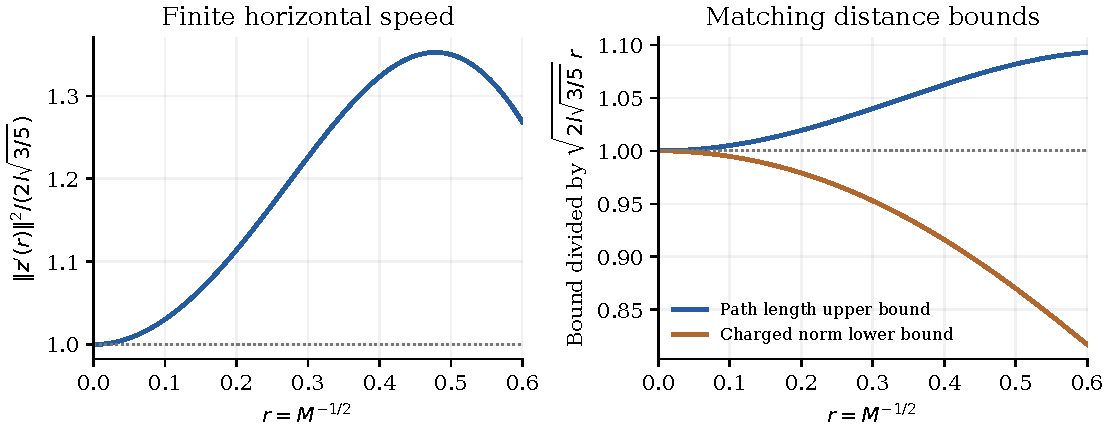
\includegraphics[width=\textwidth]{figures/output/boundary_geometry.pdf}
\caption{The explicit finite balanced curve, after removing its overall $l$ scale.
Left: squared horizontal speed divided by its endpoint value. Right: the
integrated path-length upper bound and charged-norm lower bound, divided by
the common leading distance. Both tend to one as $r\to0$. The curves are
finite-model calculations; the passage to the actual metric is the proved
relative estimate, not a numerical HE computation.}
\label{fig:boundary}
\end{figure}

\FloatBarrier
\begin{thebibliography}{Wue26b}

\bibitem[BiS16]{BiswasSchumacher16}
I.~Biswas and G.~Schumacher,
\emph{The Weil--Petersson current for moduli of vector bundles and applications to orbifolds},
Ann. Fac. Sci. Toulouse Math. (6) \textbf{25} (2016), no.~4, 895--917.
\href{https://doi.org/10.5802/afst.1514}{doi:10.5802/afst.1514}.

\bibitem[BuS20]{BuchdahlSchumacher20}
N.~Buchdahl and G.~Schumacher,
\emph{Polystability and the Hitchin--Kobayashi correspondence}, preprint (2020),
\href{https://arxiv.org/abs/2002.03548v1}{arXiv:2002.03548v1}.

\bibitem[CT24]{ClarkeTipler24}
A.~Clarke and C.~Tipler,
\emph{Semi-stability and local wall-crossing for Hermitian Yang--Mills connections},
J. Symplectic Geom. \textbf{22} (2024), no.~3, 673--694.
Locators refer to \href{https://arxiv.org/abs/2304.05245v1}{arXiv:2304.05245v1}.

\bibitem[Cos99]{Coste99}
M.~Coste, \emph{An introduction to o-minimal geometry},
Institut de Recherche Math\'ematique de Rennes, lecture notes, November 1999.
\href{https://perso.univ-rennes1.fr/michel.coste/polyens/OMIN.pdf}{Author notes}.

\bibitem[Cos05]{Coste05}
M.~Coste, \emph{Real algebraic sets}, lecture notes, 23 March 2005.
\href{https://perso.univ-rennes1.fr/michel.coste/polyens/RASroot.pdf}{Author notes}.

\bibitem[Del25]{Delloque25}
R.~Delloque, \emph{Continuity of HYM connections with respect to metric variations},
J. London Math. Soc. (2) \textbf{112} (2025), no.~1, e70219.
\href{https://doi.org/10.1112/jlms.70219}{doi:10.1112/jlms.70219}.
Locators refer to \href{https://arxiv.org/abs/2403.16814v4}{arXiv:2403.16814v4}.

\bibitem[Kob87]{Kobayashi87}
S.~Kobayashi, \emph{Differential Geometry of Complex Vector Bundles},
Publications of the Mathematical Society of Japan, vol.~15,
Princeton University Press, Princeton, NJ, 1987.
\href{https://www.mathsoc.jp/assets/pdf/publications/pubmsj/Vol15.pdf}{Mathematical Society of Japan edition}.

\bibitem[Man99]{manetti2005}
M.~Manetti, \emph{Deformation theory via differential graded Lie algebras},
Seminari di Geometria Algebrica 1998--1999, Scuola Normale Superiore,
Pisa, 1999; \href{https://arxiv.org/abs/math/0507284v1}{arXiv:math/0507284v1} (2005).

\bibitem[Stacks]{stacks}
The Stacks Project Authors, \emph{The Stacks Project},
\href{https://stacks.math.columbia.edu/tag/01XT}{Tag 01XT (projective-space cohomology)},
\href{https://stacks.math.columbia.edu/tag/0BED}{Tag 0BED (K\"unneth formula)}, and
\href{https://stacks.math.columbia.edu/tag/00MC}{Tag 00MC (faithfully flat completion)},
accessed October 31, 2026.

\bibitem[Wue26a]{wuebben2026three}
B.~J.~Wuebben, \emph{Hermitian--Einstein metrics and small spectra for
three-step extensions}, preprint, October 31, 2026.
\href{https://doi.org/10.5281/zenodo.23850990}{doi:10.5281/zenodo.23850990}.

\bibitem[Wue26b]{WuebbenRelativeMetrics26}
B.~J.~Wuebben, \emph{Relative metric estimates near reducible Yang--Mills connections},
preprint, October 28, 2026.
\href{https://doi.org/10.5281/zenodo.23740619}{doi:10.5281/zenodo.23740619}.

\end{thebibliography}

\end{document}
